% !TEX root = ../thesis-example.tex
%
%\chapter{Cosmological Measurements from Angular Power Spectra analysis of BOSS DR12 Tomography}
\chapter{Tomographic Analysis of BOSS DR12 Galaxy Clustering in Harmonic Space}
\label{Chap:BOSS}

\cleanchapterquote{If you’re going to try,\\
go all the way.\\
There is no other feeling like \\
that. \\
You will be alone with the gods \\
and the nights will flame with \\ 
fire.}{Charles Bukowski}{(Roll the Dice)}
\vspace*{\fill}

In this chapter, I perform an angular power spectra analysis of the Baryon Oscillation Spectroscopic Survey DR12 galaxies, a spectroscopic follow-up of around 1.3 million SDSS galaxies over 9,376 deg$^2$ with an effective volume of $\sim 6.5$ (Gpc $h^{-1}$)$^3$ in the redshift range $0.15 \leq  z  < 0.80$. I split this sample into 13 tomographic bins ($\Delta z = 0.05$); angular power spectra were calculated using a Pseudo-$C_{\ell}$ estimator. Measurements were then binned with a bandwidth of $\Delta \ell = 8$. Covariance matrices were estimated using log-normal simulated galaxy maps using the measured angular power spectra instead of a fiducial $C_{\ell}$. These were validated using a Gaussian expression for the variance of the Pseudo-$C_{\ell}$ estimator which takes into account effects introduced by the partial sky nature of the observations -- the mixing of modes due to the mask. Finally, in order to use the full shape of the angular power spectra for Cosmological analyses, I have performed null-tests of systematic contamination against eighteen different sources of systematics by using cross-correlations between the data and systematics. Apart from the larger modes -- the first bandwidth $\ell$-modes -- I have found no significant contamination from observational systematics, indicating that the full shape of BOSS DR12 angular power spectra of galaxies can be used for cosmological analysis.

\textit{The work presented in this chapter was presented in \citet{2018LoureiroBOSS}.} 

\newpage
%%%%%%%%%%%%%%%%%%%%%%%%%%%%%%%%%%%%%%%%%%%%%%%%%%%%%%%%%%%%%%%%%%%%%%%%
% 					   % INTRODUCTION %
%%%%%%%%%%%%%%%%%%%%%%%%%%%%%%%%%%%%%%%%%%%%%%%%%%%%%%%%%%%%%%%%%%%%%%%%
\section{Introduction}\label{sec:BOSS:intro}
Recent years have seen increased interest in measuring cross-correlations of distinct cosmological probes. Simultaneously modelling and fitting auto- and cross-correlations of observable cosmological fields can improve the dark energy figure-of-merit of surveys \citep{2008PhRvD..77l3525W}, provide better control of systematic errors, and potentially unveil new physics \citep[e.g.][]{Kirk2015}. Examples of this approach include combinations of CMB primary and secondary anisotropies with galaxy clustering and cosmic shear signals that help to constrain galaxy bias and intrinsic alignments \citep{Giannantonio2016, Hand2015}, `3x2pt' correlations between galaxy clustering and lensing signals which provide the strongest low-redshift constraints on cosmological models \citep{2017MNRAS.465.1454H, 2017arXiv170801530D}, and also between galaxy clustering and CMB \citep{2016Nicola, 2017Nicola, Doux2017}.

\qquad A consistent treatment of all probes requires a common theoretical framework for the analysis of the data and covariance matrices across the different correlations. A natural candidate for this is the angular power spectrum. It has been in widespread use by the CMB community for decades \citep{COBE,Healpix,Polspice0,PolSpiceSzapudi2001,PolSpice2001}, providing several advantages over other statistical estimators. Spherical harmonic decompositions are particularly suited to the analysis of data on the sphere, as they are easily connected to the underlying linear cosmological perturbations in a statistically isotropic and homogeneous Universe, and possess a simple covariance structure for most practical cases despite mode mixing from partial sky observations. Construction of the estimator from galaxy survey data does not require any de-projection using cosmological information, and covariance estimation from log-normal simulations can be estimated in a cosmology-independent way. This allows for a consistent end-to-end analysis. Last, but not least, self-calibration of photometric redshift distributions using cross-correlations with spectroscopic surveys is more readily implemented, and more robust to potential systematic errors \citep{McQuinnWhite2013, 2016McLeod} when compared to other methods such as $P(k)$, $\xi(r)$ and $w(\theta)$ \citep{2017RossBOSS,2017SalazarBOSSwTheta}.  In this chapter, it is argued that this should be the case because methods which live in angular space such as the method presented here and $w(\theta)$ can be naturally binned finely and hence more information about the redshift evolution can be extracted without further modelling and further assumptions. It is also further argued that non-linearities are better separated in this method that they would be if using the data in configuration space.

\qquad Spectroscopic surveys give precise information about the radial distances to galaxies, since the redshifts can be precisely measured from the spectra. In light of the precision in redshift for such galaxy surveys, the usual cosmological approach is the use the 3D power spectrum, $P(k)$, or the 3D correlation function in real space, $\xi(r)$ \citep{2001Percival,2017RossBOSS,2017BeutlerBOSS,2017WangBOSS}. Although these approaches have some advantages related to exploring the full radial information from spectroscopic surveys, a fiducial cosmology always needs to be assumed in order to translate from redshift space to real space. This choice of fiducial cosmology may potentially bias cosmological measurements, justifying once more the choice of a tomographic angular power spectra analysis.

\qquad However, there are difficulties involved in using angular power spectrum estimators on a spectroscopic galaxy survey. Firstly, it is not simple to ensure that all of this radial information is contained in the angular power spectra of projected redshift bins - even if a fine redshift binning strategy is employed. A second and more relevant issue is that spectroscopic surveys have a much lower galaxy density due to necessarily long integration times and targeting of specific galaxies with fibre spectrographs. This leads to a low signal-to-noise ratio of galaxies to Poisson noise once the data are projected in several tomographic redshift bins. A judicious choice of redshift bin width and Fourier scales can ensure that all relevant linear cosmological information is retrieved \citep{Asorey2012, Gaztanaga2012, Eriksen2015, Kirk2015}, but no consistent application of 2D angular power spectra tomography with multiple narrow bins has been attempted on real spectroscopic survey data.\footnote{However, \citet{2017SalazarBOSSwTheta} perform a similar analysis in real space with the BOSS DR12 galaxies.}

\qquad In this work, I apply the angular power spectrum formalism to the Baryon Oscillation Spectroscopic Survey 12th and final public data release (BOSS DR12). The Baryon Oscillation Spectroscopic Survey (BOSS) is one of the components of the third phase of the Sloan Digital Sky Survey (SDSS-III). Its main aim is to measure the preferred scale of baryonic acoustic oscillations in the primordial baryon-photon plasma, as imprinted in the late-time galaxy distribution. The DR12 data release contains the largest spectroscopic catalogue to date \citep{BOSS2015}. It is based on observations of around 2.5 million objects of which around 1.5 million were classified as galaxies, which are further selected to form a large-scale structure galaxy sample ready for cosmological analysis \citep{BOSSCatalogue2016}. I decided to work with this data set because of its constraining power, its public availability, and because of the possibility of comparing my results to those previously obtained by the BOSS collaboration with this same data set (see \citealt{2016BOSSCosmology} and the BOSS publications website\footnote{http://www.sdss3.org/science/boss\underline{~~}publications.php} for a list of cosmological publications from the collaboration).

\qquad Using the BOSS large-scale structure sample, I show that it is possible not only to measure the full shape of the angular power spectra in very thin tomographic redshift bins, but also to obtain reliable cosmological constraints for $\Lambda$CDM, $w$CDM and $\Lambda$CDM with $\sum m_{\nu}$ cosmologies using such a survey alone (See Chapter \ref{Chap:BOSS-Cosmo}). The method presented here uses the full shape of the angular power spectra -- not just the BAO scale. This is achieved by separating the galaxy samples into tomographic redshift bins with $\Delta z = 0.05$, and using both the auto power spectra and the cross power spectra of adjacent bins to extract information from the radial correlation of galaxies.% Further combination with external CMB \citep{PlanckCosmology2016} and SNIa \citep{JLAdata} data sets achieves competitive constraints on the models mentioned above.

\qquad This chapter is organised as follows: Section \ref{Sec:Data} describes the BOSS LSS sample selection criteria, the mask creation, and the construction of the galaxy overdensity maps. Section \ref{Sec:Measurements} describes the Pseudo-$C_{\ell}$ estimator used for the angular power spectrum analysis. Section \ref{Sec:Theory} describes the theoretical modelling of the angular power spectrum and the use of log-normal mocks for covariance matrix estimation. Section \ref{Sec:Systm} describes the analysis of potential systematic errors using the cross-power spectra between the data and different sources of systematic effects. Finally, Section \ref{Sec:Concl1} concludes this Chapter by outlining the next steps towards probing cosmological parameters with the data-vector generated in this Chapter and used on the following Chapters. %Section \ref{Sec:CosmoBananas} explains the Bayesian modelling for cosmological parameter estimation, describes a series of consistency checks performed on the data, the covariance matrix, and the pipelines, and finally presents cosmological parameter constraints for flat $\Lambda$CDM, $w$CDM, and $\Lambda$CDM + $\sum m_{\nu}$ models using the BOSS $C_{\ell}$s alone and in combination with external CMB results from the Planck collaboration \citep{PlanckLikelihood2015} and type Ia supernovae results from JLA \citep{JLAdata}.

%%%%%%%%%%%%%%%%%%%%%%%%%%%%%%%%%%%%%%%%%%%%%%%%%%%%%%%%%%%%%%%%%%%%%%%%
% 					   			% DATA %
%%%%%%%%%%%%%%%%%%%%%%%%%%%%%%%%%%%%%%%%%%%%%%%%%%%%%%%%%%%%%%%%%%%%%%%%
\section{BOSS DR12 Data}\label{Sec:Data}
The Baryon Oscillation Spectroscopic Survey Data Release 12 (BOSS DR12) is one of the experiments from the third phase of the Sloan Digital Sky Survey (SDSS-III), providing the largest galaxy redshift survey to date. The full description of the BOSS DR12, including target selection criteria and systematics, can be found in \cite{BOSS2015}. 

\qquad The BOSS DR12 is subdivided into two main samples: LOWZ and CMASS. The BOSS Collaboration created these samples by applying colour-magnitude and colour-colour cuts to the SDSS photometric catalogue in order to generate lists of targets for spectroscopic observation. The LOWZ sub-sample is designed as a simple extension of the original SDSS Luminous Red Galaxy (LRG) sample \citep{2001Eisenstein} at low redshifts, while the CMASS  sample is defined to select a stellar mass-limited sample of galaxies of all colours - hence its name, for ``constant stellar mass" - complemented by a colour cut whose goal is to select higher-redshift objects. The targets were then observed spectroscopically and objects that revealed themselves not to be galaxies (e.g. stars or quasars) were discarded. For a comprehensive discussion of the photometric cuts, selection criteria, and the terminology used, see \cite{BOSS}.

\subsection{Galaxy Catalogues}
%\begin{wrapfigure}{r}{0.5\textwidth}
  \begin{figure}
  \vspace{-30pt}
  \begin{center}
      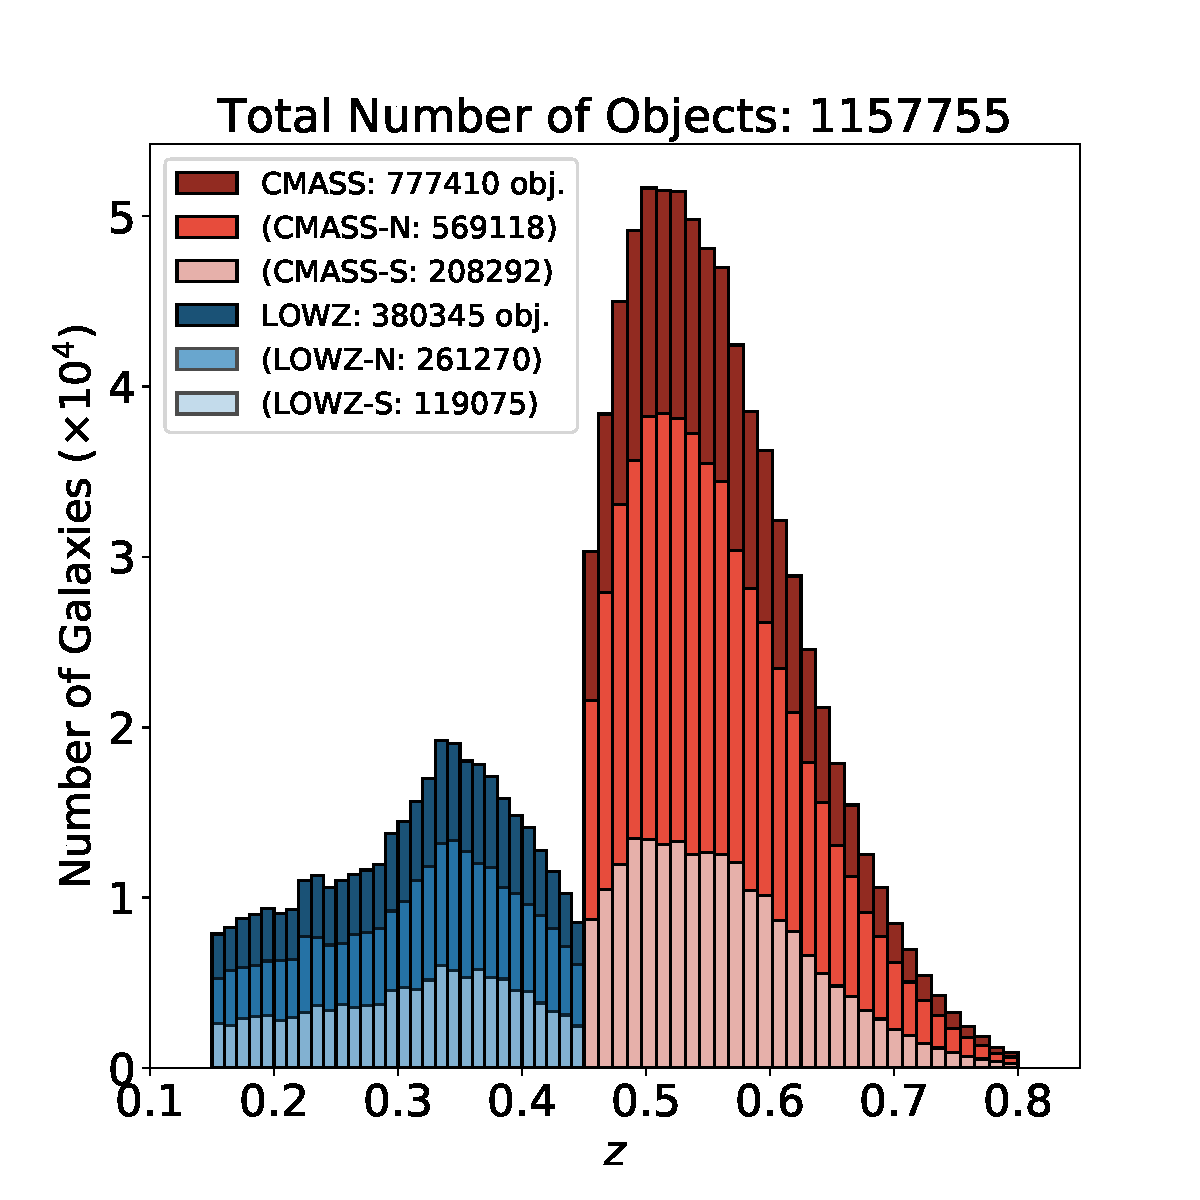
\includegraphics[scale=0.450]{BOSS-FIGS/Nz_BOSS}
      \caption[The redshift distribution of the different BOSS samples.]{The redshift distribution of the different BOSS samples. The darker histogram correspond to the total samples for LOWZ ($0.15\leq z <0.45$) and CMASS ($0.45\leq z < 0.80$). The overlap between samples was excluded using object ID, leaving a total number of 1,157,755 galaxies. Figure \ref{fig:Masks} shows the angular selection function for the samples.}
      \label{fig:NZ_BOSS}
      \end{center}
  \end{figure}
%\end{wrapfigure}
%In order to compare methods and results with the official BOSS collaboration results \citep{2016BOSSCosmology}, the construction of the catalogues in this work follows a similar procedure outlined in \cite{BOSSCatalogue2016} and the data was downloaded from the BOSS DR12 website\footnote{http://data.sdss3.org/sas/dr12/boss/}. This section outlines the main characteristics of the samples and a few differences in catalogue design tailored to the method I am using. Further details on the photometric cuts, selection criteria, and the terminology used can be found on the papers mentioned above\footnote{As mentioned, the main catalogue creation algorithm follows the algorithm outlined in \cite{BOSSCatalogue2016} and was not created by me nor any of my collaborators from Loureiro et al, \textit{in prep}.}.
To facilitate comparison of my results with the official BOSS collaboration results \citep{2016BOSSCosmology}, the construction of the catalogues used in this work followed a procedure similar to that outlined in \cite{BOSSCatalogue2016}. The data set was downloaded from the BOSS DR12 website.\footnote{http://data.sdss3.org/sas/dr12/boss/} I have further restricted these samples by applying redshift cuts of $0.15 \leq z < 0.45$ for LOWZ and $0.45 \leq z < 0.80$ for CMASS. These cuts ensure that the LOWZ and CMASS samples do not overlap in redshift, which simplifies the tomographic analysis. I use $z = 0.45$ (and not a lower $z$) as the dividing point between the two samples because the LOWZ sample has around $12\%$ more galaxies in $0.4 < z < 0.45$ than does CMASS. See figure \ref{fig:NZ_BOSS} for the resulting redshift distributions. Note also that the upper limit of $z < 0.8$ for CMASS is greater than the $z < 0.75$ limit used in \cite{BOSSCatalogue2016}. As a result of these factors the redshift ranges used in this work differ from those quoted in \cite{BOSSCatalogue2016} and \cite{2016BOSSCosmology}. Further details on the photometric cuts, selection criteria, and the terminology used can be found on the papers mentioned above\footnote{As mentioned, the main catalogue creation algorithm follows the algorithm outlined in \cite{BOSSCatalogue2016} and was not created by me nor any of my collaborators from \cite{2018LoureiroBOSS}.}. The subsections that follow outline the main characteristics of the samples.

\subsubsection{LOWZ Sample:}
The LOWZ sample is designed to contain luminous red galaxies (LRGs) with redshift up to $0.45$ as a extension of the SDSS-I/II LRG Cut I sample \citep{2001Eisenstein}. The targets are selected at low redshifts by a cut around the predicted colour locus (Equation \ref{Eq:ColourCutLZ}), and a selection of bright red objects is done at each redshift by a variable colour-magnitude cut in the \textit{r}-band (Equation \ref{Eq:RedSelecLZ}). This is the main cut in the LOWZ sample as it produces a constant number density on the redshift range of this sample. According to \cite{BOSSCatalogue2016}, the number of galaxies in the sample is extremely sensitive to this cut (see also \cite{2013ROSS}). Star-galaxy separation is done, for LRGs, with a cut on the \textit{r}-band magnitudes as shown in Equation \eqref{Eq:StarGalLZ}. Finally, to guarantee a high spectroscopic redshift success rate, a cut is performed on the \textit{r}-band to impose a brightness limit, as shown in Equation \eqref{Eq:FinalCutLZ}.

\qquad In summary, the photometric target selection criteria for the LOWZ sample is \citep{BOSSCatalogue2016}:
\begin{align}
 & |c_{\perp}| < 0.2 \label{Eq:ColourCutLZ} \\
 & r_{cmod} < 13.5 + c_{\parallel}/0.3 \label{Eq:RedSelecLZ} \\
 & r_{psf} - r_{cmod} > 0.3 \label{Eq:StarGalLZ} \\
 & 16 < r_{cmod} < 19.6 \label{Eq:FinalCutLZ}
\end{align}

\qquad In the first months of observation, the BOSS collaboration used a different star-galaxy separation criterion compared to that used later (see Appendix A from \citealt{BOSSCatalogue2016}). As a result, some sky regions from the LOWZ sample (specifically LOWZE2 and LOWZE3) have a redshift distribution that differs to that in other regions. As the method I am using relies on having a consistent redshift distribution across the sky, I excluded these regions from the LOWZ sample (see Figure \ref{fig:Masks}). 

\subsubsection{CMASS Sample:}
The CMASS sample was designed to be closer to a mass limited sample, extending the Cut-II LRGs from SDSS-I/II \citep{2001Eisenstein} to bluer and fainter objects using a sliding colour-magnitude cut as shown in Equation \eqref{Eq:CMCut2}. The cut in the quantity $d_{\perp}$ (Equation \ref{Eq:RedCutCM}) results in an increase in the number density of objects for the redshift range of $0.45 < z < 0.80$ (see Figure \ref{fig:NZ_BOSS}). Model and magnitude limit cuts (Equations \ref{Eq:CMCut3} and \ref{Eq:CMCut4}) ensure high redshift success rates while preventing low redshift objects from being erroneously targeted. Outliers and problematic blended objects are excluded using cuts in \textit{i}- and \textit{r}-band magnitudes (Equations \ref{Eq:CMCut5} and \ref{Eq:CMCutPix}). Finally, star-galaxy separation was done by performing a varying cut in $i_{psf} - i_{mod}$ and $z_{psf} - z_{mod}$ based on \cite{2006Cannon2Slaq} (Equations \ref{Eq:CMStarGal1} and \ref{Eq:CMStarGal2}).

\qquad In summary, the CMASS sample photometric target selection is \citep{BOSSCatalogue2016}:
\begin{align}
& i_{mod} < \min (19.86 + 1.6(d_{\perp}-0.8),19.9) \label{Eq:CMCut2} \\
& d_{\perp} > 0.55 \label{Eq:RedCutCM} \\
& 17.5 < i_{cmod} < 19.9 \label{Eq:CMCut3} \\
& i_{fib2} < 21.5\label{Eq:CMCut4} \\
& r_{mod} - i_{mod} < 2 \label{Eq:CMCut5} \\
& r_{dev,i} < 20.0 \text{ pix} \label{Eq:CMCutPix} \\
& i_{psf} - i_{mod} > 0.2(21-i_{mod}) \label{Eq:CMStarGal1} \\
& z_{psf} - z_{mod} > 0.46(19.8 - z_{mod}) \label{Eq:CMStarGal2}
\end{align}

\qquad Although around 25,000 galaxies were targeted with slightly different selection criteria (see Section 3.3.1 from \cite{BOSSCatalogue2016} for further details), this does not affect significantly the sample's redshift distribution (in the way that it did for LOWZE2 and LOWZE3 samples), and therefore I retain these galaxies in the sample.

\qquad Contrary from what was done in \cite{BOSSCatalogue2016} and \cite{2016BOSSCosmology}, I exclude the CMASS sample galaxies on the redshift range $0.40<z<0.45$ as the LOWZ sample has around $12\%$ more galaxies on this range, see figure \ref{fig:NZ_BOSS}. I also keep the galaxies beyond $0.75$ meaning that the redshift range I am using for CMASS is $0.45 \leq z < 0.80$ (figure \ref{fig:NZ_BOSS}). I made the first choice in order to maintain the same masks for each sample individually and in order to minimise any potential systematic effect due to redshift distributions. The second choice is made due to the way I deal with the low number of galaxies beyond $ z > 0.75$. These result in a different redshift range for CMASS and LOWZ than the ones quoted on the papers aforementioned.

\subsubsection{Total Galaxy Weights:}\label{Sec:GalWeights}
Various observational effects, such as fibre collisions, will introduce bias into clustering statistics calculated from raw DR12 data. To offset this, the BOSS collaboration provides a weighting scheme for each object; clustering statistics calculated using object counts weighted by this scheme are then expected to be unbiased by such effects. The scheme is described in \cite{BOSSCatalogue2016}, which in turn was based on \cite{2014Anderson}. In this work, I use the same weighting scheme:

%In order to obtain the correct unbiased clustering information from the galaxy catalogues, I apply the same weighting scheme proposed by \cite{BOSSCatalogue2016}, which was based on \cite{2014Anderson}. This weighting is provided on the catalogues downloaded from the BOSS DR12 website and are a combination of stellar density, seeing, redshift failures, fibre collisions and close-pair corrections:
\qquad For each targeted galaxy the BOSS collaboration provides three components to the weighting scheme, corresponding to different observational effects \citep{BOSSCatalogue2016,2014Anderson}:
\begin{itemize}
\item{$w_{\text{systot}}$, a combination of stellar density with airmass, sky flux, reddening, and other seeing conditions;}
\item{$w_{\text{cp}}$, which is due to close-pair objects, i. e., objects that can not have both their spectra measured due to fibre collisions;}
\item{$w_{\text{noz}}$, which takes into account nearest neighbours following a redshift failure by up-weighting such galaxies.}
\end{itemize}
Following Equation 50 in \cite{BOSSCatalogue2016}, one can combine these into a single weight for each galaxy:

\begin{equation}
w_{\text{tot,i}} = w_{\text{systot,i}}(w_{\text{cp,i}}+w_{\text{noz,i}}-1) \ .
\label{Eq:Weights}
\end{equation}

The default values of $w_{\text{cp}}$ and $w_{\text{noz}}$ are unity. By construction the term inside the parentheses in Equation \eqref{Eq:Weights} conserves the total number of targeted galaxies. A more detailed study of the impact of observational systematics is presented in Section \ref{Sec:Systm}.

\subsection{Masks and Map making}\label{Sec:MaskMaps}
In this section, I describe the final data products construction -- maps and masks -- I create using the \healpix\footnote{\url{http://healpix.sourceforge.net}} software \citep{Healpix}. The procedures I outline in this section are followed for both CMASS and LOWZ in the same way.

\subsubsection{Masks and Angular Selection Function:}\label{Sec:Masks}
%------------------------------------------------------------------------%
%                        		MASKS
%------------------------------------------------------------------------%
\begin{figure}
\begin{subfigure}{.5\textwidth}
  \centering
  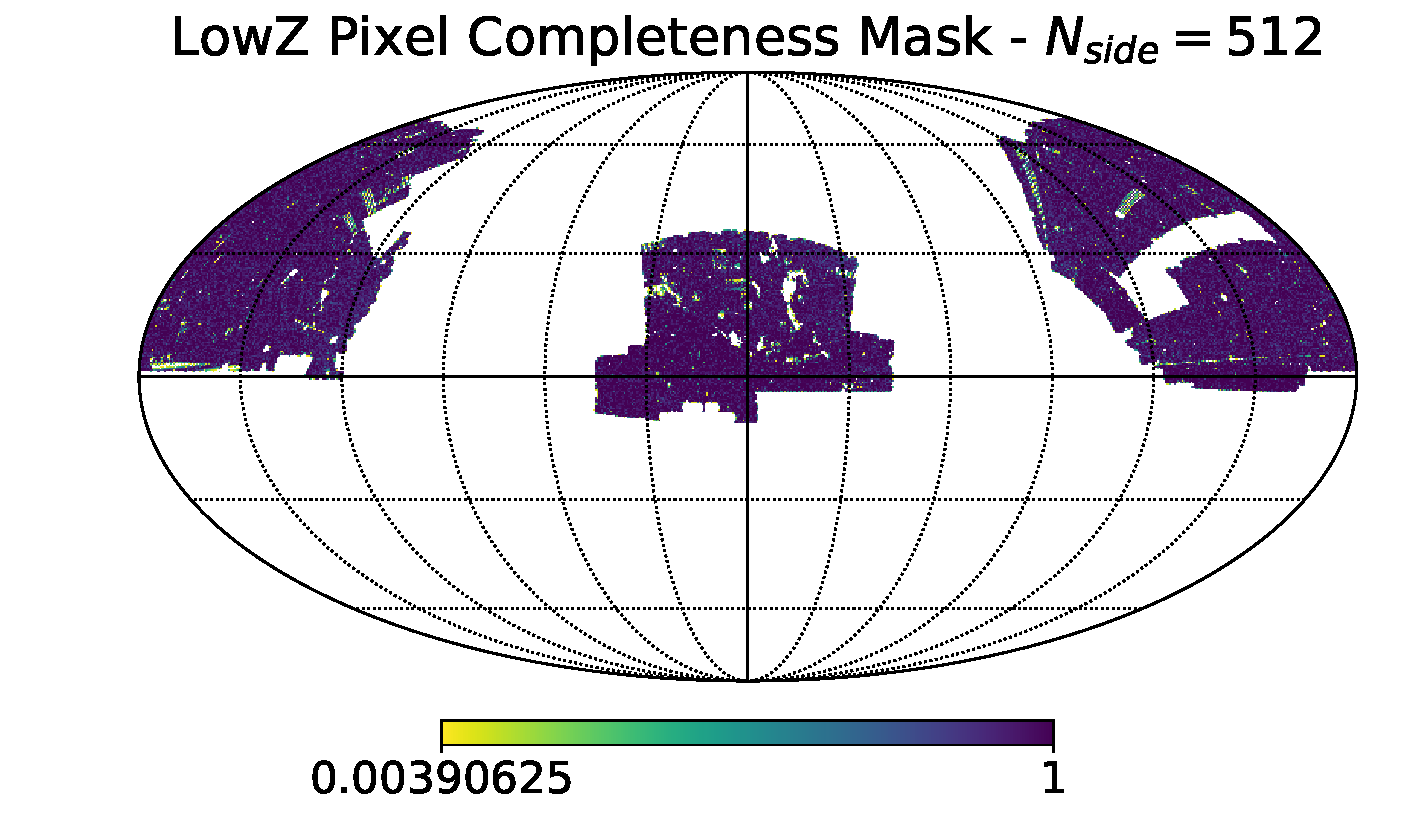
\includegraphics[width=\linewidth]{BOSS-FIGS/LOWZ_Mask}\label{fig:LOWZ_Mask}
\end{subfigure}%
\begin{subfigure}{.5\textwidth}
  \centering
  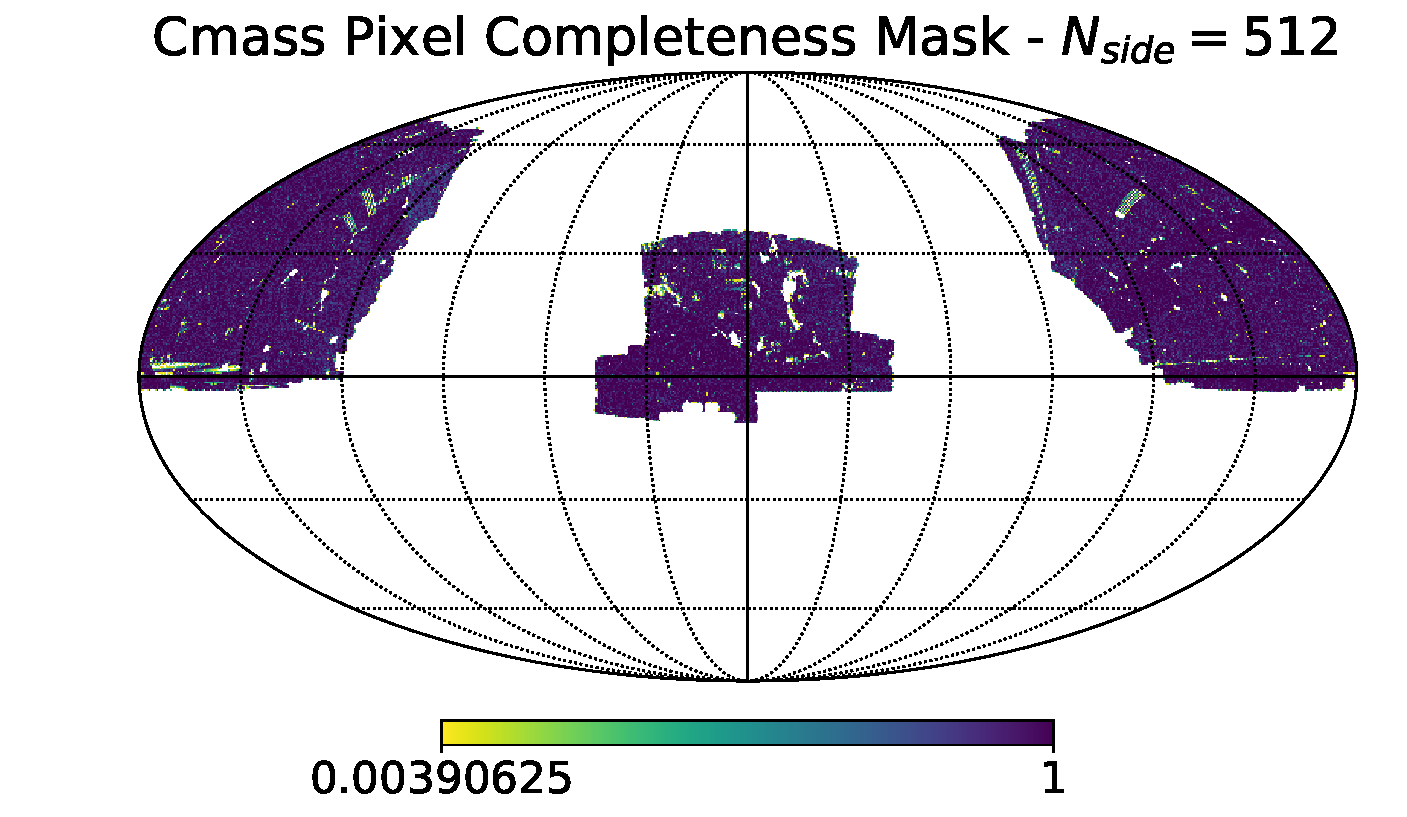
\includegraphics[width=\linewidth]{BOSS-FIGS/CMASS_Mask}\label{fig:CMASS_Mask}
\end{subfigure}
\caption[LOWZ and CMASS angular selection function masks.]{{\small \textit{(left)} LOWZ final pixel completeness angular mask with $N_{side}= 512$. I excluded the LOWZE2 and LOWZE3 regions (the holes in the NGC) due to the non-standard $N(z)$ in these regions (the result of an initially different observing strategy that affected these regions). After performing a pixel completeness cut of $0.8$, the total used area of the mask is around $8529.58\deg^2$ ($f_{sky} = 0.2067$). \textit{(right)}  CMASS final pixel completeness angular mask with $N_{side}=512$. After performing a pixel completeness cut of $0.8$, the total used area of the mask is around $9444.63\deg^2$ ($f_{sky} = 0.2286$). }}
\label{fig:Masks}
\end{figure}

The BOSS collaboration provides\footnote{\url{http://data.sdss3.org/sas/dr12/boss/lss/}} an acceptance mask and several veto masks; these are in \mangle format \citep{2008Mangle}. The acceptance mask is continuous (i.e., takes values between 0 and 1), the value for a given region reflecting the completeness of observations there; in other words, the extent to which spectra were obtained for all targets. The precise value is given by:

% The BOSS collaboration team provides the \mangle \citep{2008Mangle} acceptance and veto masks based on the completeness of each observed tilling, centerpost collisions, collision priority, bright stars, bright objects, seeing cuts, extinction cuts, and other observational factors (for more details, check section 5.1 from \cite{BOSSCatalogue2016}). I downloaded the \texttt{MANGLE} files from the BOSS database \footnote{\textsf{http://data.sdss3.org/sas/dr12/boss/lss/}} and converted the great circle coordinates from the \texttt{MANGLE} polygons to declination and right ascension in order to convert it to a \texttt{HEALPIX} pixelisation scheme using a $N_{side}$ of 8192 ($N_{pix} = 12\times N_{side}^2$). The acceptance mask and the veto masks are then merged at this high resolution \texttt{HEALPIX} scheme, and a hard cut is performed on the completeness of the acceptance mask, $C_{BOSS} > 0.7$, before merging them -- accepted pixels = 1; rejected pixels = 0.
\begin{equation}
C_{BOSS} = \frac{N_{obs}+N_{cp}}{N_{obs}+N_{cp}+N_{\text{missed}}} \ ,
\end{equation}

\noindent where:

\begin{itemize}
\item $N_{obs}$ is the number of spectroscopically observed objects including galaxies, stars, and unclassified objects; 
\item $N_{cp}$ is the number of close-pair objects;
\item $N_{\text{missed}}$ is the number of targeted objects with no spectra.
\end{itemize}

\qquad The veto masks are binary maps (i.e., regions are marked as either good or bad); these maps mask out regions affected by observational factors such as centerpost collisions, collision priorities, bright stars, bright objects, seeing cuts, extinction cuts, and others (see Section 5.1 in \cite{BOSSCatalogue2016}).

\qquad The BOSS acceptance and veto masks are transformed into a high resolution \healpix pixelisation with $N_{side} = 16384$. Using this pixelisation scheme, I combine the BOSS masks to yield a high resolution binary mask. This is done by accepting pixels in which the acceptance mask value $C_{BOSS}$ exceeds 0.7 and which are not marked as bad in any of the veto masks; other pixels are rejected. This choice of completeness cut is based on the BOSS LSS catalogue algorithm from \cite{BOSSCatalogue2016}. This high resolution binary mask is then degraded to a lower resolution ($N_{side} = 512$) continuous mask with values $C_{pix}$ (the \textit{pixel completeness factor}), defined for a given pixel to be the fraction of high resolution sub-pixels that are marked as good in the high resolution binary mask. This is the final mask product and can be seen in figure \ref{fig:Masks} for LOWZ and CMASS. The masks used for the pseudo angular power spectrum estimator (PCL) measurements in Section \ref{Sec:Measurements} contains a hard cut in $C_{pix} \geq 0.8$: values $< 0.8$ are set to 0 and values $\geq 0.8$ are set to 1.

%------------------------------------------------------------------------%
%                        		MAP MAKING
%------------------------------------------------------------------------%
\begin{table}
\centering
\caption[Tomographic redshift bins limits, number of galaxies, and shot-noise levels.]{Details of each redshift tomographic bin containing information on redshift limits, number of objects, and shot-noise value. Note that the shot-noise is calculated after applying the galaxy weights (Section \ref{Sec:GalWeights}, equation \eqref{Eq:Weights}).}
\label{Tb:Shells}
\begin{tabular}{lllcl}
\hline
\hline
Sample Bin & $z_{min}$ & $z_{max}$ & \# of galaxies & Shot-Noise \\ & & & & (gal/strd)$^{-1}$ \\
\hline 
\hline
LOWZ--0  & 0.15      & 0.20      &   43,265   & $6.143 \times 10^{-5} $\\
LOWZ--1  & 0.20      & 0.25      &   51,271   & $5.156 \times 10^{-5} $\\
LOWZ--2  & 0.25      & 0.30      &   59,713   & $4.416 \times 10^{-5} $\\
LOWZ--3  & 0.30      & 0.35      &   85,394   & $3.064 \times 10^{-5} $\\
LOWZ--4  & 0.35      & 0.40      &   83,537   &  $3.136\times 10^{-5} $\\
LOWZ--5  & 0.40      & 0.45      &   57,165   &  $4.605 \times 10^{-5} $\\
CMASS--6 & 0.45      & 0.50      &   177,383  &  $1.577\times 10^{-5} $\\
CMASS--7 & 0.50      & 0.55      &   217,636  &  $1.275\times 10^{-5}$ \\
CMASS--8 & 0.55      & 0.60      &   179,571  &  $1.545\times 10^{-5}$ \\
CMASS--9 & 0.60      & 0.65      &   114,398  &  $2.435 \times 10^{-5}$ \\
CMASS--10 & 0.65      & 0.70      &   57,537   &  $4.850 \times 10^{-5}$ \\
CMASS--11 & 0.70      & 0.75      &   23,631   &  $1.182 \times 10^{-4}$ \\
CMASS--12 & 0.75      & 0.80      &    7,253   &  $3.839 \times 10^{-4}$\\
\hline
\hline
\end{tabular}
\end{table}

\subsubsection{Healpix overdensity maps:}\label{Sec:Maps}
%From the galaxy catalogues, the final data products to be used in the analysis are galaxy overdensity \texttt{HEALPIX} maps. In order to produce them, first I properly bin both data catalogues into redshift tomographic bins of $\Delta z = 0.05$. This results in 6 tomographic bins for LOWZ, from $z \geq 0.15$ to $z=0.45$; and 7 tomographic bins for CMASS, from $z \geq 0.45$ to $z = 0.80$. Details about each redshift bin can be found in table \ref{Tb:Shells}. Next, using \texttt{HEALPIX}'s \texttt{ANG2PIX} function, I create a \textit{weighted number counts} map which contains the number of objects in each \texttt{HEALPIX} pixel, $n_p$, weighted by the \textit{total galaxy weight} given by equation \eqref{Eq:Weights}. To create the final galaxy overdensity maps, I need to up-weight the $n^g_p$ maps according to the pixel completeness from the masks, $C_{pix}$ -- a second and different up-weighting than the one presented in Section \ref{Sec:GalWeights}. Here, objects in pixels with $C_{pix} <  0.8$ are now considered outside the footprint, \textit{i. e.} the pixel value is set to zero. Thus, the expression for the overdensity maps is:
 From the galaxy catalogues, I generate the final data products to be used in the analysis: the galaxy overdensity \healpix maps. First, I bin both data catalogues into tomographic redshift bins of $\Delta z = 0.05$. This gives six tomographic bins for LOWZ ($0.15 \leq z < 0.45$) and seven for CMASS ($0.45 \leq z < 0.80$). Details about each redshift bin can be found in table \ref{Tb:Shells}. According to \cite{Asorey2012}, $\Delta z = 0.05$ is the thickest possible redshift bin size a spectroscopic redshift survey with $z < 1$ can have in order to keep sufficient radial information without suppressing the radial BAO information due to averaging originating from mode projection. Smaller bin sizes could improve the quality of radial information; however, the trade-off between bin size and shot-noise per bin for the case considered in this chapter is such that the shot-noise would then be too high for the considered scales. The use of the cross-power spectra between adjacent bins allows for RSD information to be properly probed as explained in Section \ref{Sec:RSD}.

\qquad Next, I create a \textit{weighted number counts} map which contains the number of objects in each \healpix pixel, $n_p$, weighted by the \textit{total galaxy weight} ($w_{tot}$) given by Equation \eqref{Eq:Weights}. To create the final galaxy overdensity maps, I up-weight the maps by the inverse of the pixel completeness factor from the masks, $C_{pix}$. Here, objects in pixels with $C_{pix} <  0.8$ are now considered outside the footprint, i.e. the pixel value is set to zero. Thus, the expression for the overdensity maps is:

\begin{equation}
\delta_{z,p}^g = 
\begin{cases}
\left(\frac{1}{C_{pix,p}}\frac{n^g_{z,p}}{\bar{n}_z}\right) - 1 & \text{, if } C_{pix,p} > 0.8 \\
0 & \text{, otherwise}
\end{cases}
\label{Eq:OverDMaps}
\end{equation}
where $\bar{n}_z$ is the mean number of weighted galaxies per observed pixel, in each redshift tomographic bin. Note that the weight I am referring here are the one mentioned in Equation \ref{Eq:Weights}, the $\bar{n}_z$ is not weighted by the pixel completeness weight.  After these procedures are applied to all 13 redshift tomographic bins, the data products are ready for the power spectra of these maps to be measured using the Pseudo-$C_{\ell}$ estimator described on the next sections.

%------------------------------------------------------------------------%
%                      EESTIMATORS AND MEASUREMENTS
%------------------------------------------------------------------------%
\section{Angular Power Spectra Estimators and Measurements}\label{Sec:Measurements}
The first proposed method for estimating the angular power spectrum $C_{\ell}$  \citep{Peebles1973} consists of projecting the density field onto the celestial sphere, decomposing this projected field into spherical harmonics, and then analysing statistically the coefficients of this decomposition. I refer here to this method of estimating the power spectrum as a \textit{pseudo power spectrum estimator} (PCL). This is a widely used tool for both galaxy clustering and CMB analysis and explored in several different approaches in the literature (see before-mentioned works).

\subsection{Pseudo-$C_{\ell}$ Estimator}\label{Ref:PCL}

Here, I describe the PCL estimator, following recent approaches as presented in e.g. \cite{ScharfLahav1992}, \cite{FisherLahav1994}, \cite{Wright1994}, \cite{2001Huterer}, \cite{PolSpice2001}, \cite{BlakeFerreira2004}, \cite{Blake2007}, \cite{Thomas2010Neutr}, \cite{Thomas2011b}, \cite{Thomas2011}, and \cite{Ho2012}. The aim is to measure the angular power spectrum of the galaxy overdensity field, $\delta^g$. 

\qquad Let $\bar{\rho}^g$ be the average of $\rho^g$ over the sky and define the galaxy overdensity field to be  

\EQ{}{
\delta^g = \frac{\rho^g - \bar\rho^g }{\bar\rho^g } = \frac{\rho^g }{\bar\rho^g} -1,}

\noindent This field may be represented using spherical harmonic expansion:

\EQ{}{
\delta^g(\theta, \phi) = \sum_{\ell=0}^{\ell_{max}} \sum_{m=-\ell}^{\ell} d_{\ell m} Y_{\ell m}(\theta, \phi),}

\noindent where the spherical harmonic coefficients $d_{\ell m}$ are defined by

\EQ{}{
d_{\ell m} = \int \delta^g(\theta,\phi) Y_{\ell m}^*(\theta,\phi) d\Omega.}

\noindent Here and in what follows, a coordinate system is fixed, $(\theta, \phi)$, for the celestial sphere; the spherical harmonic functions are defined with respect to this coordinate system. The estimator of the angular power spectrum of the data is then

\EQ{}{
\hat{D}_{\ell} = \frac{1}{2\ell +1} \sum_{m = -\ell}^{\ell} d_{\ell m}^{} d_{\ell m}^{\ast}.}

\noindent The averaging over $m$ is motivated by the assumed isotropy of the probability distribution governing the location of galaxies.

\qquad To handle the partial-sky case, let $\Omega_{tot}$ be the survey region and define

\EQ{Jlm}{
J_{\ell m} = \int_{\Omega_{tot}} \left|Y_{\ell m} \right|^2d\Omega \ .}

\noindent This is a normalization factor due to the average of modes in the partial sky coverage; note that $J_{\ell m}=1$ for a full-sky survey. There will also be a term correcting for bias introduced by the partial sky measurement. However this term is proportional to the average field value; in the case considered this average vanishes, so the bias correction need not be made. See Appendix \ref{Apx:PCL} for details. 

\qquad One can repeat this analysis for galaxy density fields $\rho^{g, i}$ and $\rho^{g, j}$ defined in tomographic bins $i$ and $j$. Combining the partial sky effect and tomographic binning results in an estimator $\hat{D}_{\ell}^{i j}$ for the cross- $(i \neq j)$ or auto- $(i = j)$ power spectrum of the data

\EQ{D_hat}{
\hat{D}_{\ell}^{i j} = \frac{1}{2\ell +1} \sum_{m = -\ell}^{\ell}D^{ij}_{\ell m}}

\noindent where

\EQ{D_lm_ij} {
D^{ij}_{\ell m} = \frac{\Re(d_{\ell m}^i d_{\ell m}^{j \ast})}{J_{\ell m}}.
}

\noindent Here, I take the real part $\Re()$ of a quantity whose expectation value will have no imaginary part. 

\qquad In reality one works with a pixelised celestial sphere and measure not $\rho^g$ but rather a galaxy count $n^g_p$ per pixel $p$. From this one can derive the per-pixel galaxy overdensity

\EQ{define_delta_p}{
\delta^g_p = \frac{n^g_p}{\Delta \Omega_p} \frac{\Delta \Omega_{tot}}{n^g_{tot}} - 1,}

\noindent where $n^g_{tot}$ is the total galaxy count, $\Delta \Omega_p$ the solid angle subtended by pixel $p$, and $\Delta \Omega_{tot}$ the total solid angle of the survey region $\Omega_{tot}$.

\qquad On the pixelated sphere, the spherical harmonic coefficients are estimated by

\EQ{AlmPix}{
d_{\ell m} = \sum_p \delta^g_p Y_{\ell m}^{\ast}(\theta_p,\phi_p) \Delta\Omega_p ,}

\noindent where $(\theta_p,\phi_p)$ are the coordinates at the centre of pixel $p$, $\Delta\Omega_p$ is the area of $p$, and the sum is over all pixels in the survey region.

\qquad Pixelisation is a smoothing operator, and hence suppresses power at small scales. I now summarise here the standard treatment of this effect; see \cite{Healpix,Boris2013} and the \healpix documentation for details\footnote{For details on the pixel window function: \url{https://healpix.jpl.nasa.gov/html/intronode14.htm}}. Consider the contribution of a given pixel $p$ to $d_{\ell m}$ both for the (measured) pixelised field and for the (desired) ideal continuous field; the ratio of these quantities is 

\EQ{}{
w_{\ell m}^p = \frac{\int_p Y_{\ell m}(\theta,\phi) d\Omega}{Y_{\ell m}(\theta_p,\phi_p) \Delta \Omega_p}.}

\noindent This quantity depends sensitively on $\ell$: for small $\ell$, $Y_{\ell m}$ is slowly varying and hence $w_{\ell m}^p$ will be close to unity while for large $\ell$ the rapidly varying $Y_{\ell m}$ will have vanishing integral over $p$. However the dependence on $m$ and $p$ will be small and can be averaged out (in quadrature), yielding:

\EQ{}{
w_{\ell}^2 = \frac{1}{N_{pix}(2\ell+1)} \sum_{p,m} \left| w_{\ell m}^p \right|^2.}

\noindent The ratio of the power spectra of the (measured) pixelised overdensity field to that of the (desired) continuous field will then be $w_{\ell}^2$. This study uses a \healpix resolution of $N_{side} = 512$; which means that at $\ell_{max} = 510$ this ratio of powers ($C_{\ell}^{pix}/C_{\ell}^{unpix}$) is then $0.911$ due to the pixel window function.

\qquad Galaxy clustering observations contain both signal and (Poisson) noise; spatial variations in the latter contribute to the measured auto power spectrum and this effect must be removed when estimating the power spectrum of the underlying signal. 

\qquad As the signal and noise are uncorrelated, the angular power spectra of the signal ($S_{\ell}$), data ($D_{\ell}$) and noise ($N_{\ell}$) are related by:

\EQ{SignalNoise}{
S_{\ell} = D_{\ell} - N_{\ell}.}

\qquad For most tomographic bins one can approximate the angular power spectrum of the noise as the variance of a Poisson distribution:

\EQ{NoiseNl}{
N_{\ell} \approx \frac{\Delta\Omega_{tot}}{n^g_{tot}} = \frac{1}{\bar{n}},}

\noindent where $\bar{n}$ is the mean number of galaxies per steradian.

\qquad Amending \eqref{Eq:D_hat} to account for pixelisation and shot-noise yields an estimator $\hat{S}^{ij}_{\ell}$ for the partial sky signal power spectrum between two redshift bins \textit{i} and \textit{j}:

\EQ{Sl_wl}{
\hat{S}^{ij}_{\ell} = \frac{1}{w_{\ell}^2} \left[ \left(\frac{1}{(2\ell+1)}\sum_{m=-\ell}^{\ell} D^{ij}_{\ell m}\right) - N_{\ell}\delta_{ij}\right].}


\noindent The estimator is symmetric in $i$ and $j$. Note also that there is no shot-noise contribution for the cross-power spectra ($i \neq j$). The PCL estimator described here uses galaxy overdensity maps instead of the galaxy counts maps used in \cite{Blake2007,Thomas2011} and others; Appendix \ref{Apx:PCL} describes the correspondence between the two approaches. This estimator is unbiased \citep{Peebles1973} but does not have minimum variance: maximum likelihood estimators such as QML \citep[e.g.][]{Efstat2004} have smaller variance. However, these maximum likelihood estimators are computationally expensive to use; this is why this work uses PCL. %The same is valid for the Bayesian estimator considered in chapter \ref{chap:BPL} and some extra complications related to extracting cosmological information from its full posterior are also discussed in the relevant chapter.

\begin{figure*}
\begin{center}
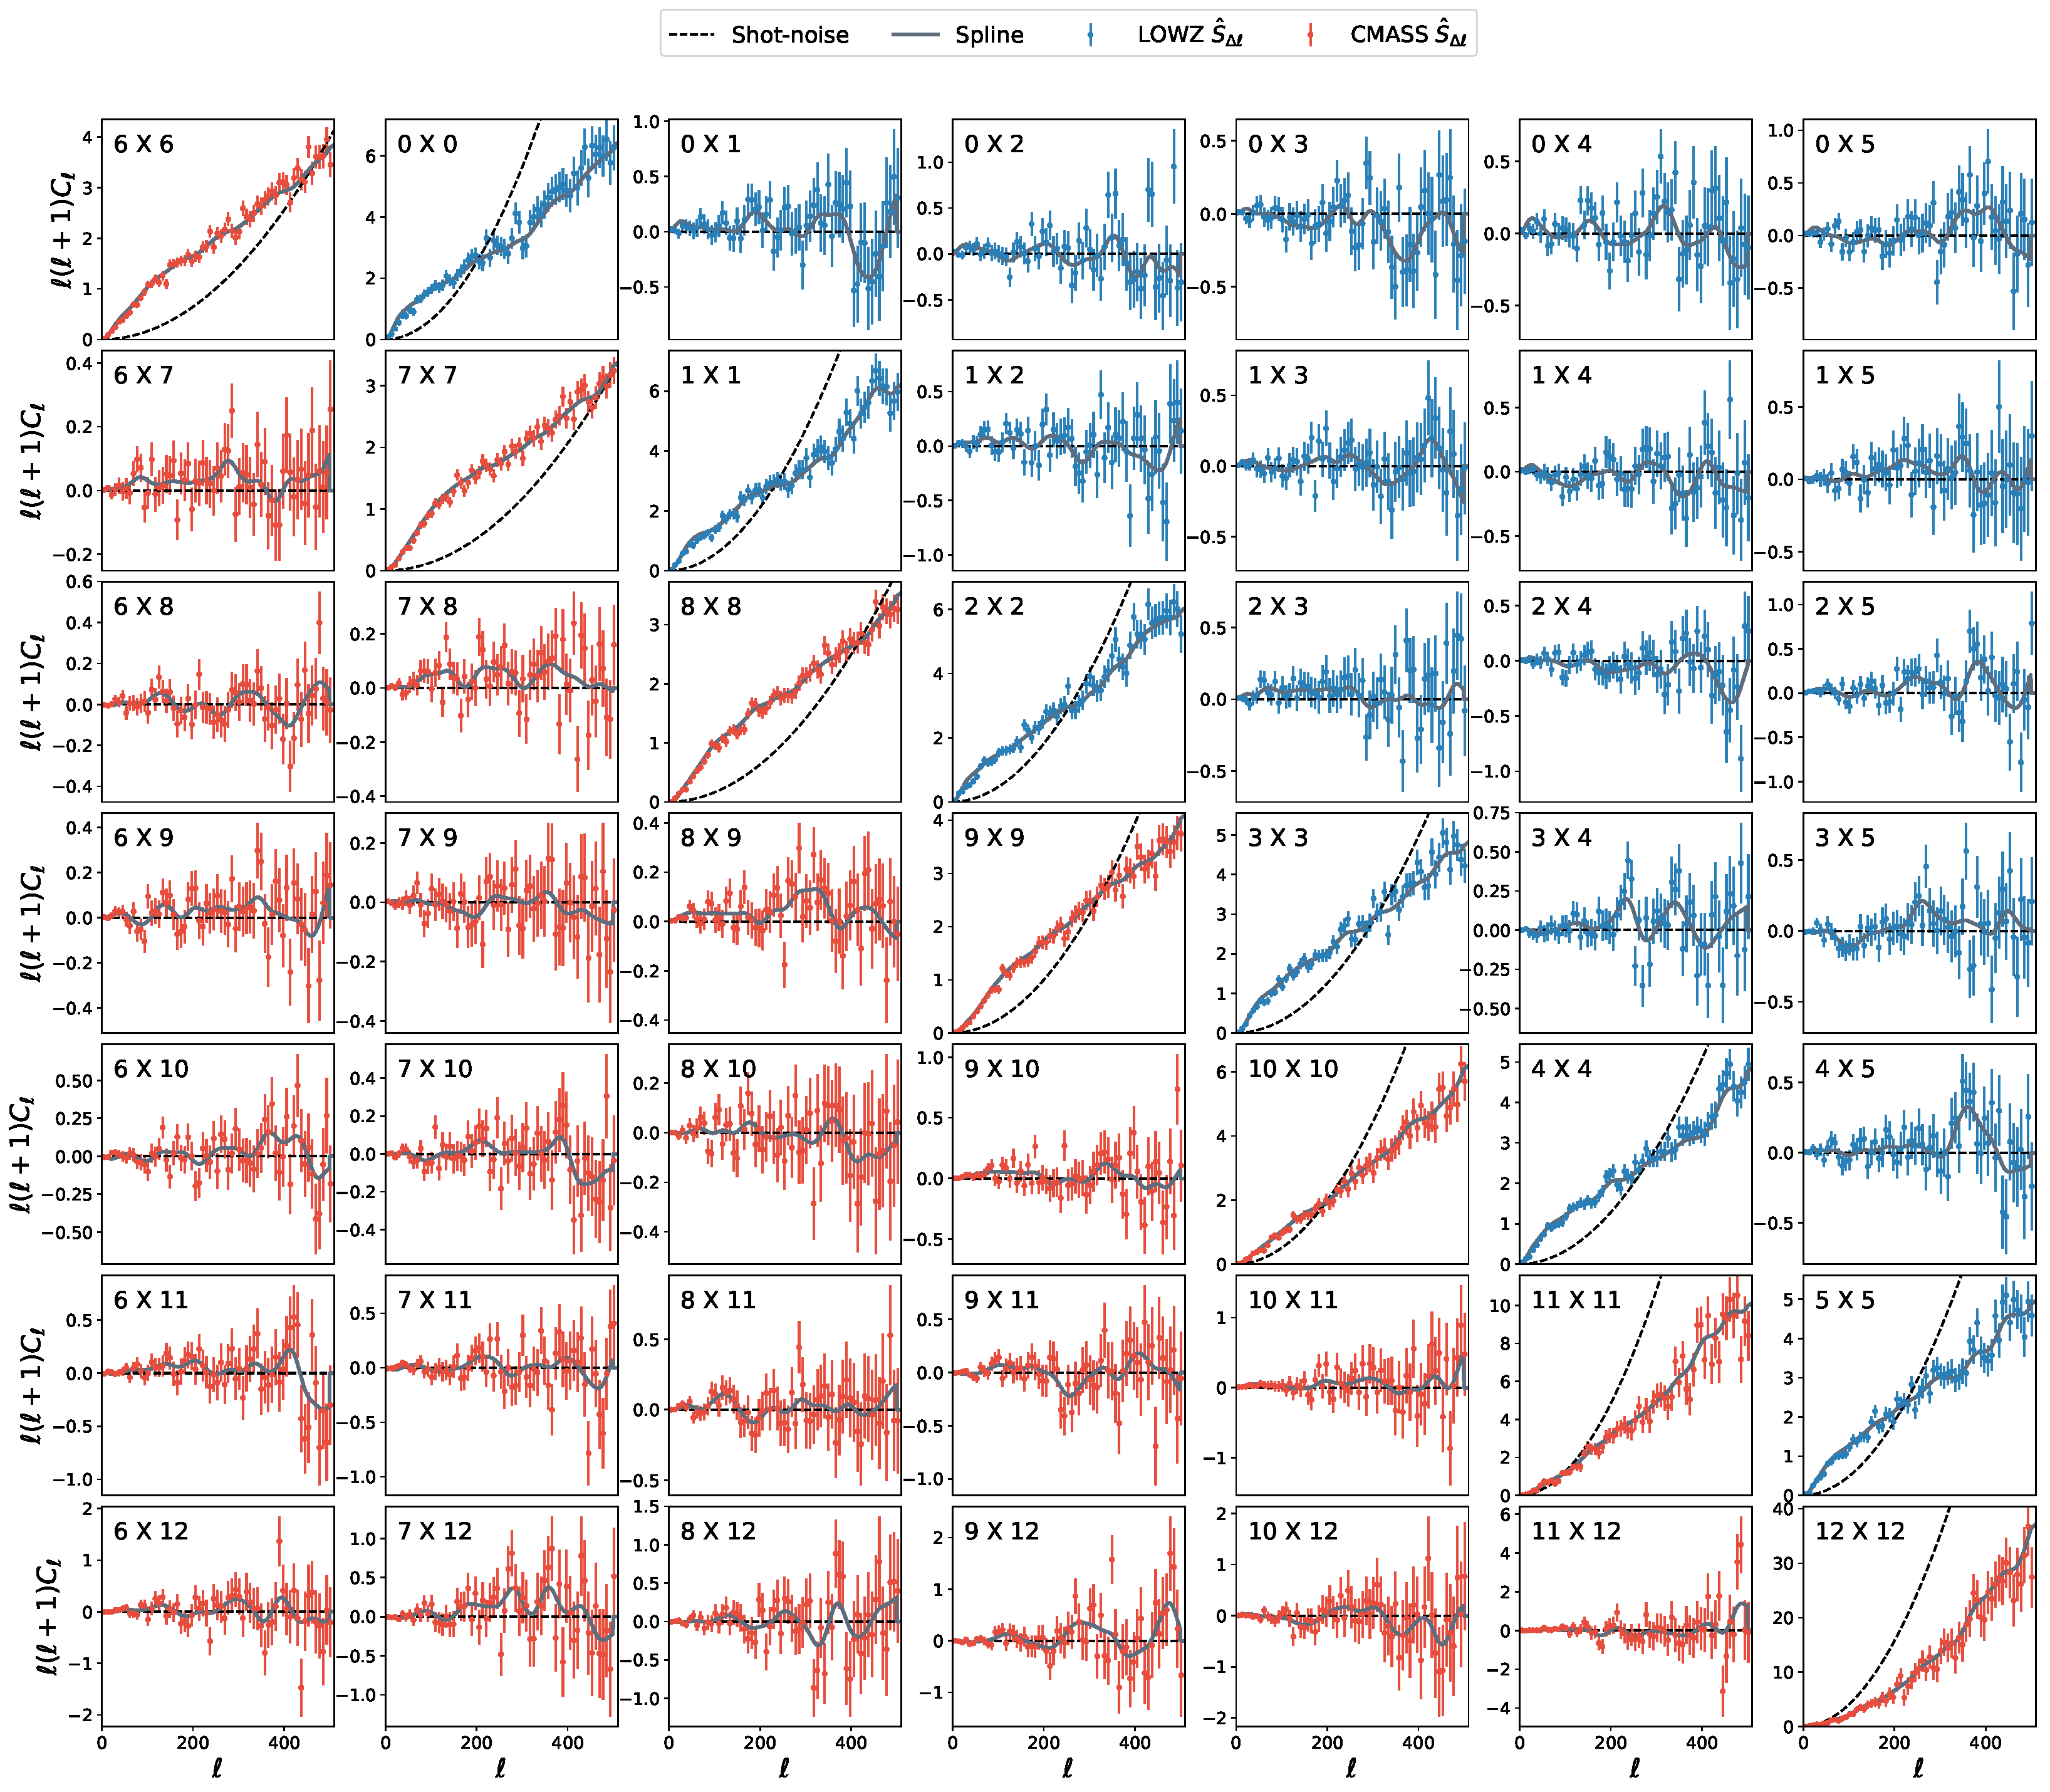
\includegraphics[width=1.0\textwidth]{BOSS-FIGS/PCL-data_red3.pdf}
\caption[Measured angular power spectra from the BOSS samples.]{Measured signal auto- and cross-power spectra for the LOWZ (blue) and CMASS (red) samples (Equation \ref{Eq:S_delta_ell}). The black dashed lines show the estimated Poissonian shot-noise (Equation \ref{Eq:NoiseNl}). The solid grey line shows the deconvolved spline used in Section \ref{Sec:Cov} to generate the log-normal mocks for covariance matrix estimation from which the error bars in this figure were estimated. Even though the measured $\hat{S}_{\Delta\ell}$ had the shot-noise removed, note that the last two CMASS bins have a significant part of their signals below the level of Poissonian shot-noise.}
\label{fig:PCLs}
\end{center}
\end{figure*}

\subsection{Bandwidth Binning and Measurements}

The measurements are binned in $\ell$ using bins of width $\Delta\ell = 8$ (so e.g. the first bin is $2 \leq \ell \leq 9$). For each bin, I calculate a weighted average of the $\hat{S}_{\ell}^{ij}$ (weighted by the number of spherical harmonic coefficients):

\EQ{S_delta_ell}{
\hat{S}_{\Delta\ell}^{ij} = \frac{\sum_{\ell \in \Delta\ell}(2\ell+1)\hat{S}_{\ell}^{ij}}{\sum_{\ell \in \Delta\ell}(2\ell+1)} \ .}

\noindent This binning acts on the measurement in a way that decorrelates mixed modes (that arise from the convolution of the true measurement and the survey's angular window function). 

\qquad Finally, I measure the PCL estimator up to $\ell_{max} = 510$; Figure \ref{fig:PCLs} shows the results for the auto- and cross-power spectra for LOWZ and CMASS. Note that I do not consider in this work any cross-correlations between the two samples; therefore, each sample is treated individually. The figure also shows error bars given by the diagonal of the covariance (estimated in Section \ref{Sec:Cov}), as well as the splines used to generate the log-normal mocks (Section \ref{Sec:Cov}). The figure shows that the last two CMASS bins are dominated by shot-noise (due to their small density of galaxies). Uncertainty in the characterisation of this noise will be included into the theoretical forward modelling presented in Section \ref{Sec:Theory} and marginalised over during the cosmological parameter estimation (Section \ref{Sec:CosmoBananas}).



%------------------------------------------------------------------------%
%                      THEORY CLS AND COVARIANCE MATRIX
%------------------------------------------------------------------------%
\section{Theory Modelling and Covariance Matrix Estimation}\label{Sec:Theory}
This work's goal is to use observations to constrain cosmological parameters; as part of this, I describe the theory that connects the statistics of the underlying matter field with the measured angular power spectra. My approach is similar to that found in the literature \citep{ScharfLahav1992,2001Huterer,Padm2007,Thomas2011,Asorey2012}.

\qquad In this section, I outline the framework necessary to obtain the desired cosmological parameter's constraints from the measured angular power spectra.  I detail here the theoretical framework used to estimate the theory vector, the procedure used to build covariance matrices from log-normal mocks, and the theoretical expression for the covariance of the PCL estimator.

\subsection{Theoretical Angular Power Spectra}
Let $\delta_{g}(\textbf{x},z)$ denote the galaxy density function. Let $\delta_{g}(\textbf{k},z)$ be its Fourier transform; one can write this in terms of the growth function $D(z)$, the bias $b(z)$ (assumed here to be scale-independent), and the Fourier components $\delta(\textbf{k},0)$ of the underlying matter distribution at the current time:

\begin{equation}
\delta_g(\textbf{k},z) = D(z)\delta_g(\textbf{k}) = D(z)b(z)\delta(\textbf{k},0).
\end{equation}

%\noindent The correlation structure of the Fourier transform is
\noindent The correlation structure of the Fourier transform is

\begin{equation}
\langle \delta_{g}(\textbf{k},z) \delta_{g}^*(\textbf{k}',z) \rangle = (2\pi)^3\delta^{(D)}(\textbf{k}-\textbf{k}')P_g(k,z) \
\end{equation}

\noindent where $P_g(k,z) = b(z)^2P(k,z)$ is the power spectrum of the galaxy density field and $P(k,z)$ is the power spectrum of the underlying matter density field. 

\qquad Integrating the galaxy density along the line of sight, $\hat{\textbf{n}}$, yields:

\begin{equation}
\delta_g(\hat{\textbf{n}}) = \int_0^\infty \delta_g(\chi(z)\hat{\textbf{n}}, z) n(z) dz
\end{equation}
%\begin{ceqn}\begin{equation}
%\delta_g^{2D}(\ell) = i^l\int \frac{d^3k}{(2\pi)^3}\delta(z,\textbf{k})W_{g,\ell}(k).
%\label{Eq:Delta2D}
%\end{equation}\end{ceqn}
where $n(z)$ is the normalised redshift-dependent selection function and $\chi(z)$ is the comoving distance. The spherical harmonic components $a_{\ell m}$ of this projected galaxy distribution are:

\begin{align}
a_{\ell m} &= \int Y_{\ell m}(\hat{\textbf{n}}) \delta_g(\hat{\textbf{n}}) d\Omega \\
		&= \int Y_{\ell m}(\hat{\textbf{n}}) \int \delta_g(\chi(z)\hat{\textbf{n}},z) n(z) dz d\Omega \\
        &= \frac{4\pi}{(2\pi)^3} \int b(z)n(z)D(z) \int \delta(\textbf{k},0) i^{\ell} j_{\ell}(k\chi(z)) Y_{{\ell},m}(\hat{\textbf{k}}) d^3k dz.\label{Eq:ThisOne}
\end{align}
where $j_{\ell}(k\chi(z))$ are the Spherical Bessel functions \citep{Thomas2010Neutr, Thomas2011}.

\begin{figure}
\begin{center}
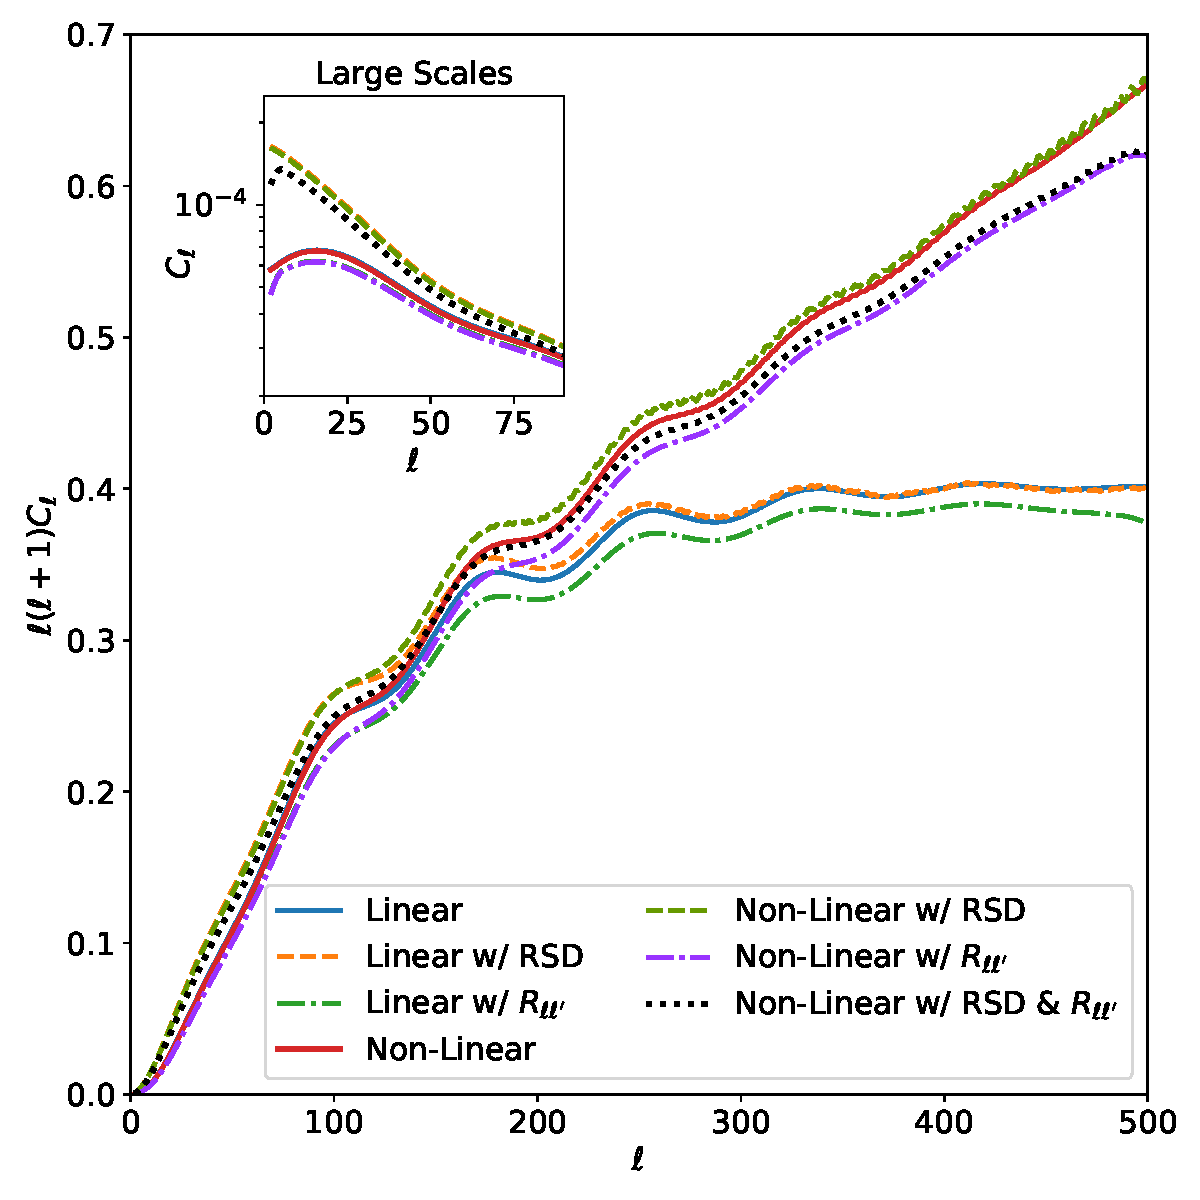
\includegraphics[width=\textwidth]{BOSS-FIGS/Cls-Comparison.pdf}
\caption[Different effects which affect the angular power spectrum modelled into \texttt{UCLCL}.]{A series of different effects which affect the angular power spectrum ($0.45 < z \leq 0.50$) in a variety of ways. The two \textit{solid lines} show the linear and non-linear $C_{\ell}$'s (Section \ref{Sec:NonLin}) which diverge as a function of scale, $\ell$. \textit{Dashed lines} include the Redshift space distortions effect (Section \ref{Sec:RSD}) which increases the power for larger scales (see sub-panel). \textit{Dot-dashed lines} show the effect of the mixing matrix convolution (Section \ref{Sec:MixingMat}) which tends to suppress power in all scales. Finally, the black dotted line is a combination of all such effects: RSDs, non-linearities, and mixing matrix convolution. The input parameters for these calculations were done using a flat cosmology: $b=1$, $h = 0.6725$, $\Omega_b = 0.0492$, $\Omega_{cdm} = 0.265$, $w_0=-1.0$, $\tau_r = 0.079$, $\log A_s = 3.093 \times 10^{-10}$, $n_s = 0.965$. These theory lines were all generated using the \uclcl code.}
\label{fig:Cl_Theory}
\end{center}
\end{figure}

\noindent The final step uses the plane wave expansion and the spherical harmonic addition theorem. One may collect the $z$ dependencies from Equation \eqref{Eq:ThisOne} into a window function:

\begin{equation}
W_{g,\ell}(k) = \int b(z) n(z)D(z)j_{\ell}(k\chi(z)) dz.\
\end{equation}

\qquad Using the window function in Equation \eqref{Eq:ThisOne} yields a simple expression for the angular power spectrum:

\begin{align}
C_{\ell}^{ij} & \equiv \left\langle a_{\ell m}^i a_{\ell m}^{j*} \right\rangle \\
& = \frac{2}{\pi} \int W^i_{g,\ell}(k)W^j_{g,\ell}(k)k^2 P(k,0) dk.
\label{Eq:ClTheoretical}
\end{align}

\noindent Here I have introduced superscripts $i$ and $j$ to denote different redshift shells and the equation above, therefore, defines both auto-$C_{\ell}$ (for $i = j$) and cross-$C_{\ell}$ (for $i \neq j$). The same formalism can be used to obtain the $C_{\ell}$ between two different tracers, between photometric and spectroscopic redshift shells, etc.

\qquad In this work, I used the Unified Cosmological Library for $C_{\ell}$s, or \uclcl code (Cuceu et al, in prep). This code obtains the primordial power spectra and transfer functions from the \class Boltzmann code \citep{Class}, and then applies Equation \eqref{Eq:ClTheoretical} to obtain the angular power spectrum. \uclcl deals with the redshift distribution in more flexible ways than does \class and \camb \citep{CAMB}: it allows for the input $n(z)$ distribution to be a spline and also allows it to be convolved with a Gaussian error function to take into account redshift systematic effects (Equation \ref{Eq:GaussianErrNz} in Section \ref{Sec:SpecNz}). {A comparison between these codes is presented in Appendix \ref{Apx:Code_Comparison}.} %which uses the \texttt{CLASS} Boltzmann code \citep{Class} to obtain the primordial power spectra and transfer functions, and project it to obtain a angular power spectrum as in equation \eqref{Eq:ClTheoretical}. Differently from \class and \camb, \uclcl deals with the redshift distribution in more flexible ways. Among which, \uclcl allows for the input $n(z)$ distribution to be a spline and also to convolve it with a gaussian error function to take into account redshift systematic effects (Equation \ref{Eq:GaussianErrNz} in section \label{Sec:SpecNz}).

%------------------------------------------------------------------------%
%                        RSD AND WINDOW FUNCTION
%------------------------------------------------------------------------%
\subsubsection{Spectroscopic Redshift Distribution and shot-noise modelling:}\label{Sec:SpecNz}
The spectroscopic selection provides a full (un-normalised) $n(z)$ function for both LOWZ and CMASS samples (see Fig. \ref{fig:NZ_BOSS}). Binning is achieved by hard cuts on each of these samples in intervals of $\Delta z = 0.05$ (Section \ref{Sec:Maps}), with no overlap or gaps between bins. Despite the impressive precision of spectroscopy, to suggest that these bins have no overlap (i.e. there is no error in the spectroscopic measurement) is unrealistic, and has a significant impact on the cross correlations between bins. Spectroscopic errors are modelled within the distribution functions by a convolution with a narrow Gaussian function representing the uncertainty on a given measurement. Such a convolution is given by
\begin{equation}
n^i(z) = \int n_*^i(z-z^\prime) e^{-\frac{z^{\prime 2}}{2\sigma_s^2}} \mathop{dz^\prime},
\label{Eq:GaussianErrNz}
\end{equation}
where $n_*^i(z)$ is the raw redshift distribution, $\sigma_s$ (the variance of the Gaussian) is a proxy for the spectroscopic measurement error, and $n^i(z)$ is the final redshift distribution to be used in calculations. In practice, the convolution is achieved by means of a fast Fourier transform (FFT) algorithm, multiplication of the functions, and reverse transform in the \uclcl pipeline.

\qquad This convolution can also be used to approximate a separate effect and more dominant effect, the so called Fingers-of-God (FoG) effect \citep{Percival-FoG2011}; which will actually dominate the measurements on $\sigma_s(z)$ in Equation \eqref{Eq:GaussianErrNz}. This is a form of redshift-space distortion (RSD) which arises as a result of random motions of galaxies within virialised structures, which elongates the appearance of structure in redshift space, i.e., it smears out the redshift distribution by the addition of Doppler shift to cosmological redshift. The convolution width $\sigma_s$ models the combined impact of spectroscopic redshift errors and of the FoG effect; $\sigma_s$ is then varied and marginalised over during the cosmological analysis. Due to the sensitivity of the cross-angular power spectra to these effects, a separate $\sigma_s$ is used for each redshift bin (for more details see Section \ref{Sec:LikelihoodsPriors}).

\subsubsection{Redshift Space Distortions:}\label{Sec:RSD}
The full large scale structure window function needs to take into account Redshift Space Distortions (RSD) \citep{Blake2007,Padm2007,Thomas2011}. This effect tends to increase the power for large scales, $\Delta \ell < 60$, due to the mix of redshift and peculiar velocities of galaxies. This local peculiar motion of galaxies creates the illusion that the ones moving towards us appear closer (i. e., they appear to be at lower redshifts); while galaxies with peculiar motion moving away from us, appear to be ever further away (i. e., they appear to be at lower at higher redshifts). This effect can be easily taken into account by adding the RSD window function  \citep{ScharfLahav1992, FisherLahav1994, Kirk2015, 2016McLeod} to equation \eqref{Eq:ClTheoretical}:

\begin{equation}\label{Eq:Window_counts}
W^{Tot,i}_{\ell}(k) = W^i_{g, \ell}(k) + W^i_{RSD,\ell}(k) \ , 
\end{equation}

where the RSD window function is given by \citep{ScharfLahav1992, Padm2007,Ho2012,Kirk2015}:

\begin{equation}
\begin{split}
%W^i_{RSD,\ell}(k) = & \beta^i \int n^i(z)D(z)\left( \frac{d\chi(z)}{dz} \right)^{-1} \times \\ & \left[ \frac{(2\ell^2 + 2\ell -1)}{(2\ell + 3)(2\ell -1)}j_{\ell}(kz) \right. \\
W^i_{RSD,\ell}(k)  = & \frac{\beta^i}{k} \int d\chi \frac{dn^i}{d\chi} j'_{\ell}(k\chi (x)) \\
 = & \beta^i \int \, n^i(\chi(z))\left[ \frac{(2\ell^2 + 2\ell -1)}{(2\ell + 3)(2\ell -1)}j_{\ell}(k\chi(z)) \right. \\
& \left. + \frac{\ell(\ell-1)}{(2\ell-1)(2\ell+1)}j_{\ell-2}(k\chi(z)) -  \dfrac{(\ell+1)(\ell+2)}{(2\ell+1)(2\ell+3)}j_{\ell+2}(k\chi(z)) \right] d\chi \ ,
\end{split}
\end{equation}

where the redshift distortion parameter, $\beta^i = (d \ln D(z)/d\ln a)/b^{i}(z) \approx \Omega_m^{\gamma}/b^i(z)$, is defined to be dependent on the bias of the given redshift shell or tracer. The RSD window function does not account for the FoG effect, which affects small scales due to the virial motion of galaxies inside clusters \citep{Kang2002}; instead, as discussed in \ref{Sec:SpecNz}, the FoG effect is subsumed into the spread of the spectroscopic redshift distribution.  

\qquad Figure \ref{fig:Cl_Theory} shows the impact on the angular power spectrum of different effects considered in this section: redshift space distortions, non-linearities, and partial sky convolution with the mixing matrix. Some of these effects affect the angular power spectrum from different scales in different redshift ranges consider in this work.

%------------------------------------------------------------------------%
%                        	NON-LINEAR C(L)
%------------------------------------------------------------------------%
\subsubsection{Non-Linear Angular Power Spectra: Halofit}\label{Sec:NonLin}
In the \uclcl pipeline, the $C_{\ell}$ estimation may be extended some way into the non-linear regime by introducing the scale-dependent non-linear overdensity in Fourier space, $\delta_{NL}(k,\chi)$, and therefore the corresponding non-linear growth function 

\begin{equation}
D_{NL}(k,\chi) = \frac{\delta(k,\chi)}{\delta(k,0)}.
\end{equation}
The calculation of this non-linear density is extracted from the \textsc{class} code (see \cite{Class,CLASSgal}), which expresses a ratio

\begin{equation}
R_{NL}(k,\chi) = \frac{\delta_{NL}(k,\chi)}{\delta(k,\chi)} = \left( \frac{P_{NL}(k,\chi)}{P(k,\chi)} \right)^{\frac{1}{2}}
\end{equation}
of the non-linear perturbations to the linear ($\delta_L(k,\chi)$), the second equality follows from $P = \langle \delta \delta^* \rangle$. This ratio is calculated using the modified \textsc{halofit} of \cite{2012-Halofit} (also employed by \textsc{camb sources} \citep{CambSources}), with additional corrections from \cite{Bird2012} for neutrino effects. 

\qquad The window function in equation \ref{Eq:Window_counts} contains both the selection function \emph{and} the growth function, which tracks the ratio of the power spectrum at different redshifts. The non-linear power spectrum is related to the linear, present day power spectrum by:

\begin{equation}
\begin{split}
P_{NL}(k,\chi) & = R^2_{NL}(k,\chi) P(k,\chi) \\
& = R^2_{NL}(k,\chi) D^2(\chi) P(k,0).
\end{split}\end{equation}

This means that the window functions in equation \ref{Eq:Window_counts} should have an additional factor of $R_{NL}(k,\chi)$ inside the integral over $\chi$. In the case of these very narrow spectroscopic redshift bins

\begin{equation}
R_{NL}(k,z) = R_{NL}(k,\bar{z})
\end{equation}
where $\bar{z}$ is the mean of the redshift bin, i.e., I assume that the non-linear ratios vary negligibly over the width of a single bin (but may vary between different bins). This simplifies the calculation of the window function considerably, and is a good approximation when the width of the bin is small. In this case the window functions for the redshift bins are straightforwardly related to their linear counterparts:
\begin{equation}
W^i_{NL,\ell}(k) = R_{NL}(k,\bar{z}^i)W^i_{g,\ell}(k).
\end{equation}
The rest of the calculation may proceed as usual. 

%------------------------------------------------------------------------%
%                        	MIXING MATRIX
%------------------------------------------------------------------------%
\subsubsection{Partial Sky: Mixing Matrix Convolution}\label{Sec:MixingMat}
\begin{figure}
\begin{subfigure}{.5\textwidth}
  \centering
  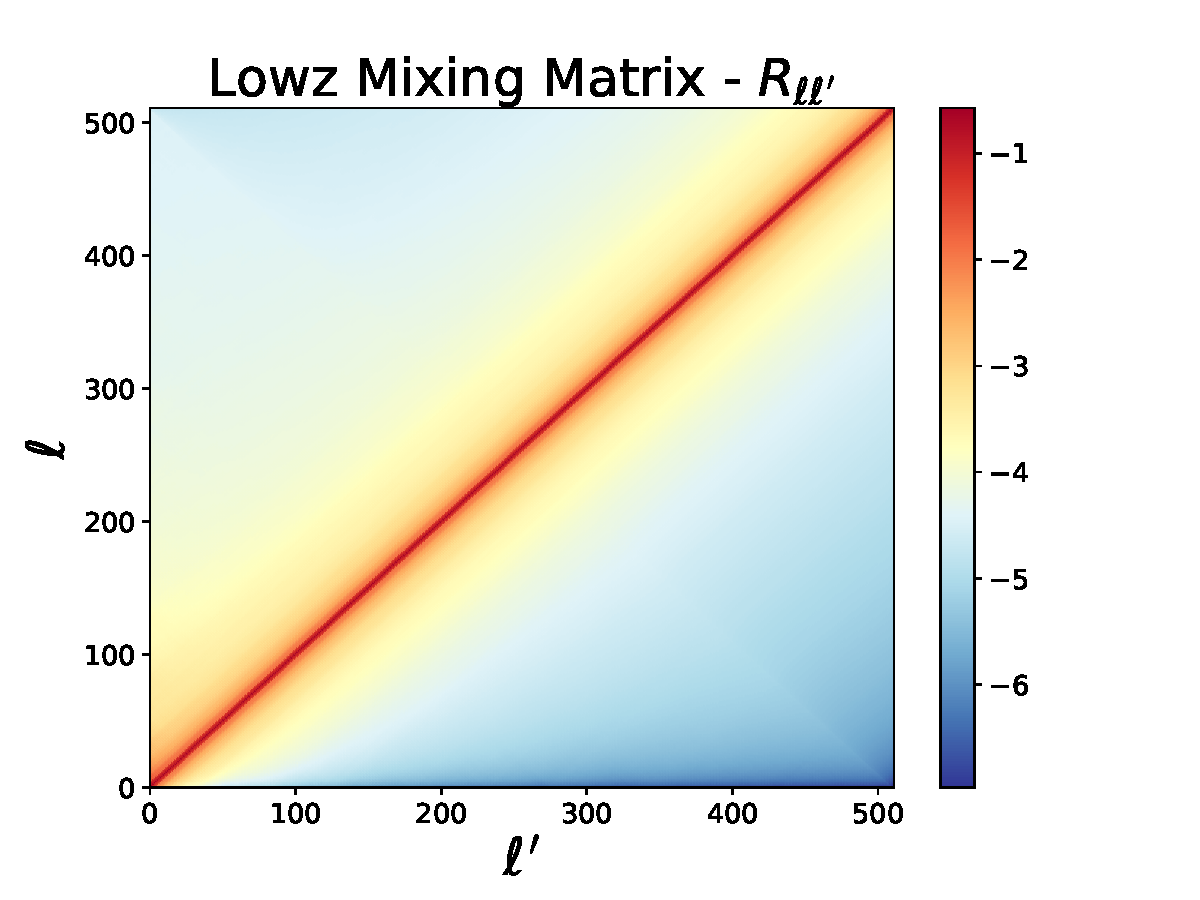
\includegraphics[width=1.2\linewidth]{BOSS-FIGS/MixMat_LOWZ}\label{fig:LOWZ_Rll}
\end{subfigure}%
\begin{subfigure}{.5\textwidth}
  \centering
  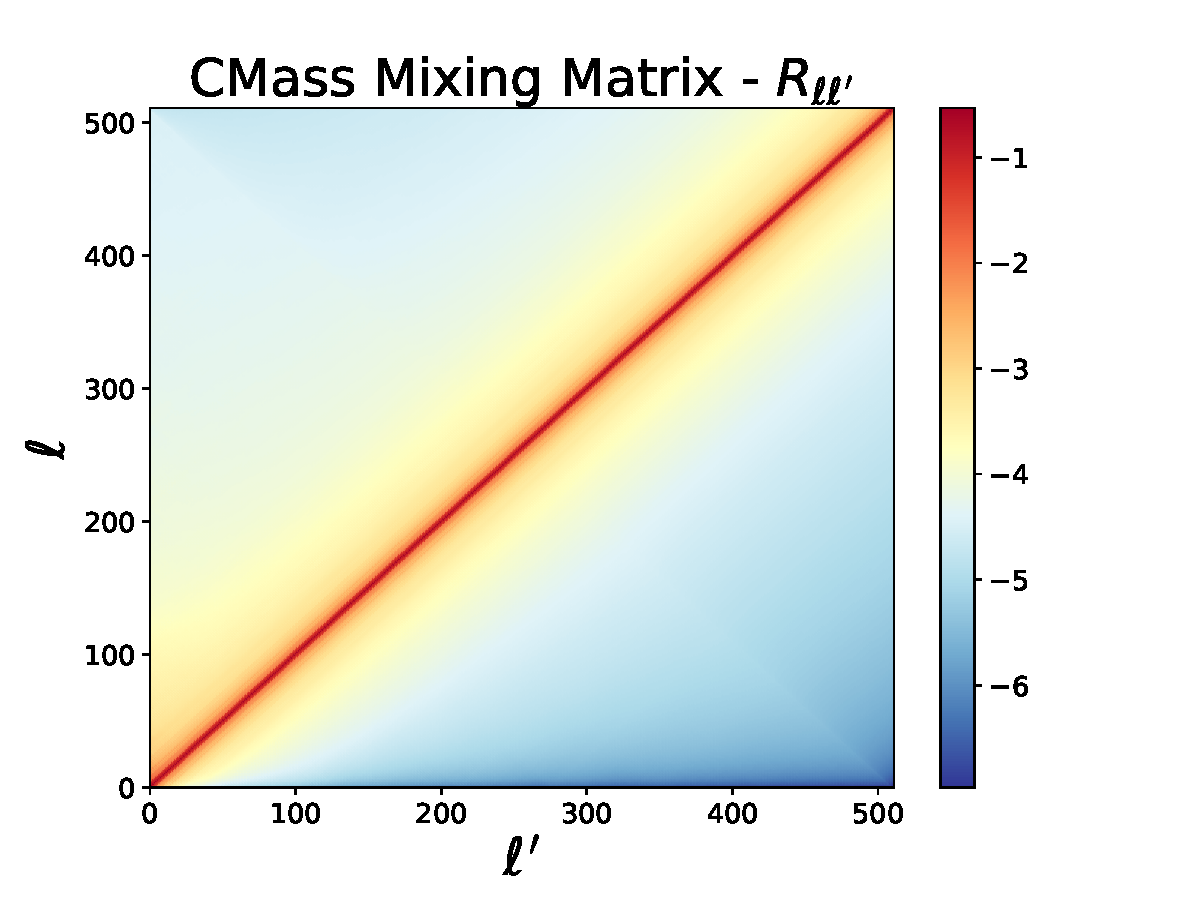
\includegraphics[width=1.2\linewidth]{BOSS-FIGS/MixMat_CMASS}\label{fig:CMASS_Rll}
\end{subfigure}
\caption[Mixing Matrix for CMASS and LOWZ.]{\textit{(left)} Mixing Matrix, $R_{\ell \ell'}$, calculated for the LOWZ mask presented in Fig. \ref{fig:Masks}. \textit{(right)} The Mixing Matrix for the CMASS mask presented in Fig. \ref{fig:Masks}, which is similar to the first one. A closer look on details for both Mixing Matrices can be seen on Fig. \ref{fig:Rll_slice}.}
\label{fig:MixMats}
\end{figure}

\begin{figure}
\begin{center}
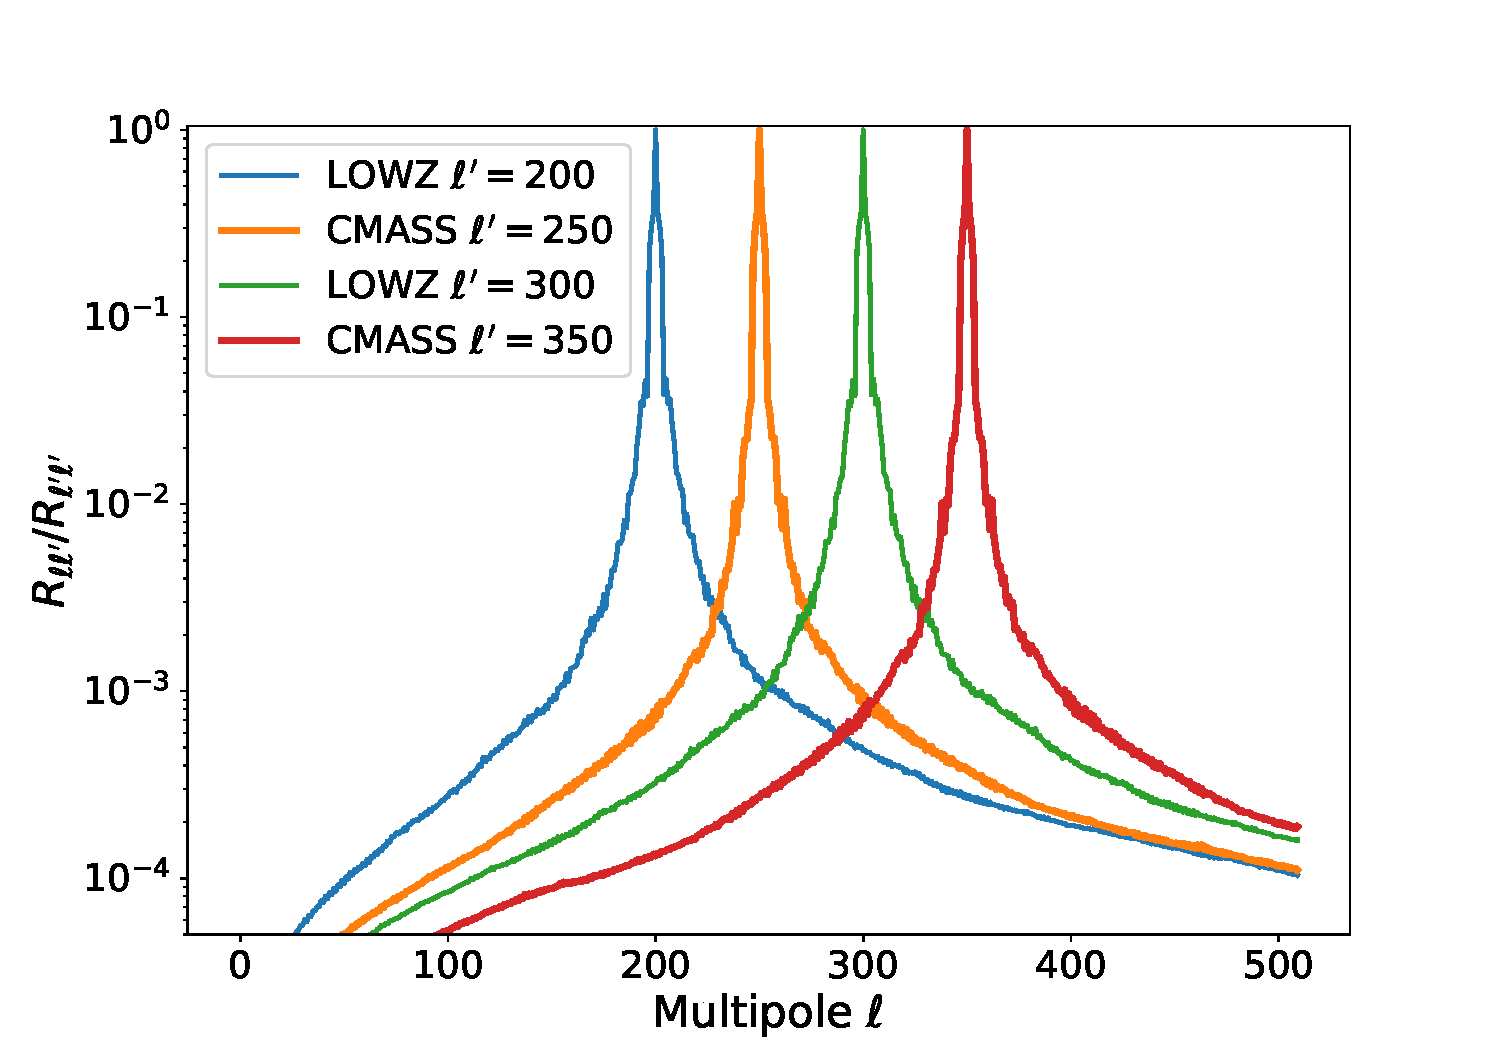
\includegraphics[scale=0.45]{BOSS-FIGS/Rll_200_300.pdf}
\caption[Slices through the Mixing Matrices.]{Slices through the Mixing Matrices (Figs. \ref{fig:MixMats}) for LOWZ (CMASS) using two different fixed multipoles values given by $\ell'=200$($250$), and $\ell'=300$($350$), where the amplitudes were normalized by $R_{\ell\ell}$. As expected, the maximum amplitude peaks in the fixed $\ell'$ and goes to zero in a given $\Delta\ell$. The profile shape of both matrices remains the same throughout the $\ell$-range, indicating the correlation introduced by the convolution with the mask on the PCL measurements presented in Fig. \ref{fig:PCLs}.}
\label{fig:Rll_slice}
\end{center}
\end{figure}

%When dealing with the PCL estimator, I perform a convolution between the theory and the survey's angular selection function effect, due to partial sky observations. As it is computationally expensive to deconvolve this effect from the measurements, this leads us to a forward modelling, where the experimental systematics are modelled and introduced into the theoretical predictions \citep{ScharfLahav1992,FisherLahav1994,Thomas2011}. This effect is taken into account through a convolution with the \textit{mixing matrix}, $R_{\ell \ell'}$ \citep{Peebles1973_2,PolSpice2001,PolSpice2005,Blake2007}:
When dealing the PCL estimator measurements, partial sky effects mean that one must calculate the convolution of the theory and the survey's angular selection function. It is computationally expensive and unstable to deconvolve this effect from the measurements. This leads to forward modelling, where the experimental systematics are modelled and introduced into the theoretical predictions \citep{ScharfLahav1992,FisherLahav1994,Thomas2011}. This effect is taken into account through a convolution with the mixing matrix, $R_{\ell \ell'}$ \citep{Peebles1973_2,PolSpice2001,PolSpice2005,Blake2007}:

\begin{equation}
S_{\ell} = \sum_{\ell'}R_{\ell \ell'} C_{\ell'} \ .
\label{Eq:Cl_Conv}
\end{equation}

\qquad The mixing matrix (see Fig. \ref{fig:Rll_slice}) itself depends only on the survey's geometry through the mask's angular power spectrum
\begin{equation}
W_{\ell} = \sum_{m=-\ell}^{\ell} \frac{|I_{\ell m}|^2}{(2\ell +1)}
\end{equation}
where (from Appendix \ref{Apx:PCL}):
\EQ{Ilm}{ I_{lm} = \sum_p^{N_{pix}} Y_{lm} (\theta_p,\phi_p)\Delta\Omega}
and the mixing matrix can be expressed as:
\begin{equation}
R_{\ell \ell'} = \dfrac{2\ell' + 1}{4\pi}\sum_{\ell ''}(2\ell'' + 1)W_{\ell ''}\begin{pmatrix} \ell & \ell' & \ell'' \\ 0 & 0 & 0 \end{pmatrix}^2.
\label{Eq:MixMat}
\end{equation}

\noindent The $2 \times 3$ matrix above is the Wigner \textit{3j} function; these coefficients were calculated using the \texttt{WIGXJPF} library \citep{Wig3j}. The mixing matrices are shown in Figure \ref{fig:MixMats} and in more detailed slices in Figure \ref{fig:Rll_slice} which gives an intuition about the size of $\Delta\ell$-bands used to bin the \textit{measured} $\hat{S}_{\ell}$s as it shows the range of multipoles that are mixed due to the survey's mask. This small correlations between the multipoles can be ``washed away" by binning the measurements. In addition, as can be seen in Figure \ref{fig:Cl_Theory}, the mixing matrix convolution tends to suppress power in all scales.

\qquad Finally, after being convolved with the mixing matrix (Equation \eqref{Eq:Cl_Conv}), the theoretical $S_{\ell}$ is then binned in the same way as the data in equation \eqref{Eq:S_delta_ell}:
\begin{equation}S_{\Delta\ell}^{ij} = \frac{1}{\sum_{\ell'}^{\ell'+\Delta\ell}(2\ell+1)}\sum_{\ell'}^{\ell'+\Delta\ell}(2\ell+1)S_{\ell}^{ij}  \ .
\label{Eq:S_delta_ell2}
\end{equation}

%------------------------------------------------------------------------%
%                       	 PCL VARIANCE
%------------------------------------------------------------------------%
\subsection{Data Theoretical Covariance}\label{Sec:TheoCov}
Here, I follow the formalism developed in \cite{2008DahlenSimons} for the covariance of spectral estimation on a sphere. For clarity I first re-derive some of the results from Section \ref{Sec:Measurements} from a different perspective, that of projectors in pixel space. 

\qquad Consider a data vector $\textbf{d}$ that is a sum of signal and noise ($\textbf{d}(\textbf{r}) = \textbf{s}(\textbf{r}) + \textbf{n}(\textbf{r})$) and that has a covariance, $\mathcal{D}$, that is a combination of signal covariance $\mathcal{S}$ and a noise covariance $\mathcal{N}$. In pixel space, the data covariance can be expressed as:

\EQ{DataCov}{\mathcal{D} = \langle \textbf{s} \textbf{s}^T \rangle + \langle \textbf{n} \textbf{n}^T\rangle = \sum_{\ell} (S_{\ell} + N_{\ell})\mathcal{P}_{\ell}}
 where $\mathcal{P}_{\ell}$ is the projector in pixel space, defined as:
 
\EQ{Projector}{\mathcal{P}_{\ell} = \sum_{m}Y_{\ell m}(\textbf{r})Y^*_{\ell m}(\textbf{r}).}
The projector satisfies the following identity in the full sky case:

\EQ{ProjIdentFullSky}{tr(\mathcal{P}_{\ell}\mathcal{P}_{\ell'}) = (\Delta\Omega_p)^{-2}(2\ell + 1)\delta_{\ell\ell'}.}
Using this identity, the Pseudo-$C_{\ell}$ estimator from Equation \eqref{Eq:Sl_wl} can be written in terms of the projector and data covariance from \eqref{Eq:DataCov}:

\EQ{}{\hat{S}_{\ell} = \frac{\Delta\Omega_p^2}{(2\ell + 1)}\left[ \textbf{d}^T \mathcal{P}_{\ell}\textbf{d} -tr(\mathcal{N}\mathcal{P}_{\ell})\right].}

\noindent where $\Delta\Omega_p$ is the area the pixels assumed to have an equal area.

\qquad Assuming a Gaussian signal \citep{Blake2007}, the covariance matrix for the angular power spectra estimator between different multipoles $\ell$ and $\ell'$ can be expressed as:

\begin{align}
\Sigma_{\ell \ell'} & = \mathcal{C}ov(\hat{S}_{\ell}, \hat{S}_{\ell'}).
\label{Eq:ThCovSimple}
\end{align}

\qquad The symmetry of the $\mathcal{P}_{\ell}$ and $\mathcal{D}$ matrices, together with the definition $\mathcal{C}ov(\textbf{X},\textbf{X}') = \langle \textbf{XX}'\rangle - \langle \textbf{X}\rangle\langle \textbf{X}'\rangle$, allows us to rewrite the covariance as:

\begin{align}
\Sigma_{\ell \ell'}& = \frac{2(\Delta\Omega_p)^4}{(2\ell+1)(2\ell'+1)}tr(\mathcal{D}\mathcal{P}_{\ell}\mathcal{D}\mathcal{P}_{\ell'})
\label{Eq:CovTrace}
\end{align}

\qquad This expression works for both full and partial sky cases. The difference between the two cases appears on the projector identity from Equation \eqref{Eq:ProjIdentFullSky}. Using the definition of the pixel space projector (Equation \ref{Eq:Projector}), the $I_{\ell m}$ expression from Equation \eqref{Eq:Ilm}, and the fact that the spectra consider in this work are \textit{moderately coloured} \footnote{\textit{Moderately coloured spectra} means that the spectra do not vary drastically within the range considered} \citep{2008DahlenSimons}, one can rewrite Equation \eqref{Eq:ThCovSimple} for a partial sky observation with area $\Delta\Omega_{tot}$ as:

\begin{align}
\Sigma_{\ell \ell'}   = & \frac{1}{2\pi}\left(\frac{4\pi}{\Delta\Omega_{tot}}\right)^2 (S_{\ell} + N_{\ell})(S_{\ell '}+ N_{\ell '}) \times \sum_{\ell ''}(2\ell ''+1)W_{\ell''}\begin{pmatrix} \ell & \ell' & \ell'' \\ 0 & 0 & 0 \end{pmatrix}^2 \\ 
& = \frac{2}{f_{sky}(2\ell' + 1)}(S_{\ell} + N_{\ell})(S_{\ell '}+ N_{\ell '})R_{\ell\ell'}
\label{Eq:CovRll}
\end{align}

where the last equality used the definition of the mixing matrix from Equation \eqref{Eq:MixMat}. Note that this expression is very similar to the one used in \cite{Blake2007,Padm2007,Thomas2011} extending it to account for the mixing of modes due to the mask. 

\qquad However, this expression (derived by \citealt{2008DahlenSimons}) does not account for the pixel window function effect nor for cross-correlations between redshift tomographic bins. In order to include these effects, I need to generalise the data angular power spectra, $S_{\ell} + N_{\ell} \rightarrow w_{\ell}^2S_{\ell}^{ij} + N_{\ell}\delta_{ij} = D^{ij}_{\ell.}$; and include the effect of cross-correlation in the covariance by changing $(S_{\ell} + N_{\ell})(S_{\ell'} + N_{\ell'})\rightarrow \frac{1}{2}[D^{ij}_{\ell}D^{ij}_{\ell'} + D^{ii}_{\ell}D^{jj}_{\ell'}]$ in Equation \eqref{Eq:CovRll} \citep{Rassat2007}. 

\qquad The final expression for the angular power spectra theoretical covariance matrix is:
\begin{align}
\Sigma_{\ell \ell'}^{ij}  = & \frac{1}{f_{sky}(2\ell'+1)}[D^{ij}_{\ell}D^{ij}_{\ell'} + D^{ii}_{\ell}D^{jj}_{\ell'}] R_{\ell \ell'} \\
= & \frac{R_{\ell\ell'}}{f_{sky}(2\ell'+1)} \left[(w_{\ell}^2S_{\ell}^{ij} + N_{\ell}\delta_{ij})(w_{\ell'}^2S_{\ell'}^{ij} + N_{\ell'}\delta_{ij}) \right. \left. + \, (w_{\ell}^2S_{\ell}^{ii} + N_{\ell}\delta_{ii})(w_{\ell'}^2S_{\ell'}^{jj} + N_{\ell'}\delta_{jj}) \right]
\label{Eq:TheoVariance}
\end{align}

and it encompasses for the Gaussian part of the covariance matrix. As in this work I do not use low-$\ell$ modes and scales beyond the non-linear regime, there is no need for further terms to be considered in the theoretical covariance estimation. It is also important to note that this expression is only used to validate the \flask covariances.

\qquad By performing the modifications mentioned above, Equation \eqref{Eq:TheoVariance} recovers the variance expression from \cite{Rassat2007}, when considering just the diagonal, for cross-power spectra; and recovers the original expression by \cite{2008DahlenSimons} when considering just the auto-power spectrum. Figure \ref{fig:Mocks_Variance} shows a comparison between the variance (the diagonal) of equation \eqref{Eq:TheoVariance} with the variance from the estimated covariance matrix from Section \ref{Sec:Cov}. Note that the covariance between different angular power spectra is considered to be zero, i. e. $\Sigma^{ij,i'j'}_{\ell\ell'} = \Sigma^{ij}_{\ell\ell'} \delta_{ii'}\delta_{jj'}$.

\begin{figure}
\begin{center}
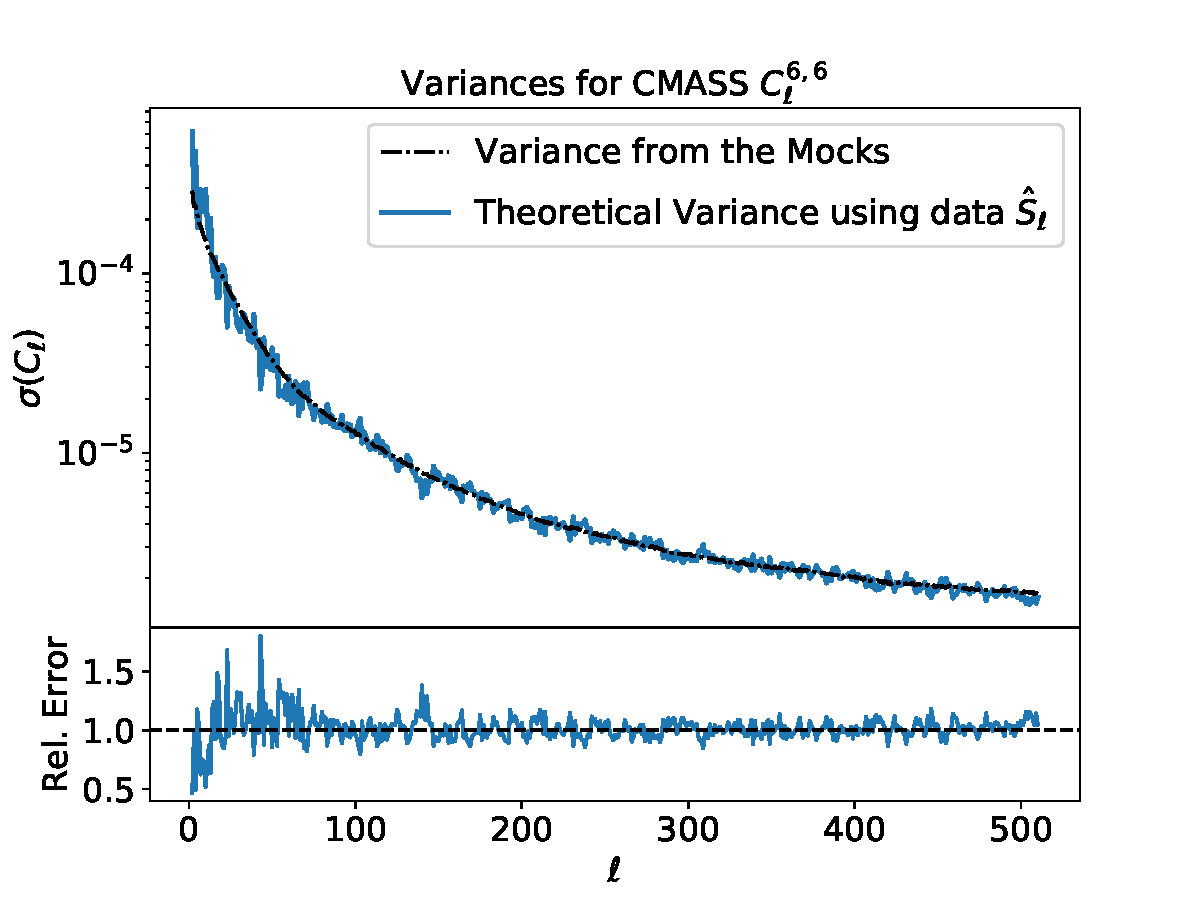
\includegraphics[scale=0.55]{BOSS-FIGS/MocksValidation.pdf}
\caption[Mock's covariance matrix validation.]{An example used for the mock's covariance matrix validation: here I compare the analytical expression for the angular power spectrum variance (Equation \eqref{Eq:TheoVariance}) with the variance from the log-normal mocks using CMASS' first auto-power spectrum as an example. The bottom panel shows the relative error for this case. This validation was checked for each one of the 42 measured $C_{\ell}$'s from fig. \ref{fig:PCLs} and no trends are apparent.}
\label{fig:Mocks_Variance}
\end{center}
\end{figure}

\subsection{Covariance Matrix using log-normal Mocks}\label{Sec:Cov}
%When obtaining cosmological parameters constrains from the PCL measurements presented in Section \ref{sec:BOSS:Measurements}, one needs reliable covariance matrices in order to estimate the measurement's errors. These covariances can be estimated using galaxy clustering mocks which reflect the cosmology, systematics effects, and any possible observational artifices that can influence the data. To do so, I use log-normal simulations instead of using Gaussian realisations \citep{Blake2007, Thomas2011} or the mocks provided by the BOSS Collaboration \citep{2016BOSSMocks}. One of the reasons why I do not make use of the official BOSS \texttt{PATCHY} mocks from \cite{2016BOSSMocks} is due to the different choice of redshift ranges for the samples: the CMASS \texttt{PATCHY} mocks do not contain galaxies beyond redshift $z_{max} \leq 0.75$ as the samples I selected go beyond this redshift range with $z_{max} \leq 0.80$ (Section \ref{sec:BOSS:data}). 
As I seek to constrain cosmological parameters using observations; one of the requirements of this process is accurate covariance matrices. Covariances can be estimated using galaxy clustering simulations that reflect not only the cosmology but also systematic effects and observational artefacts. Previous works have used either Gaussian realisations \citep{Blake2007,Thomas2011,2016Nicola} or the mocks provided by the BOSS Collaboration \citep{2016BOSSMocks,Manera2013}. However this work instead uses log-normal simulations. The decision not to use the official BOSS \texttt{PATCHY} mocks from \cite{2016BOSSMocks} was made due to the different choice of redshift ranges for the samples: the CMASS \texttt{PATCHY} mocks do not contain galaxies beyond redshift $z = 0.75$ whereas the samples I selected extend to $z = 0.80$ (as described in Section \ref{Sec:Data}). 

% \begin{figure}
% \begin{subfigure}{.5\textwidth}
%   \centering
%   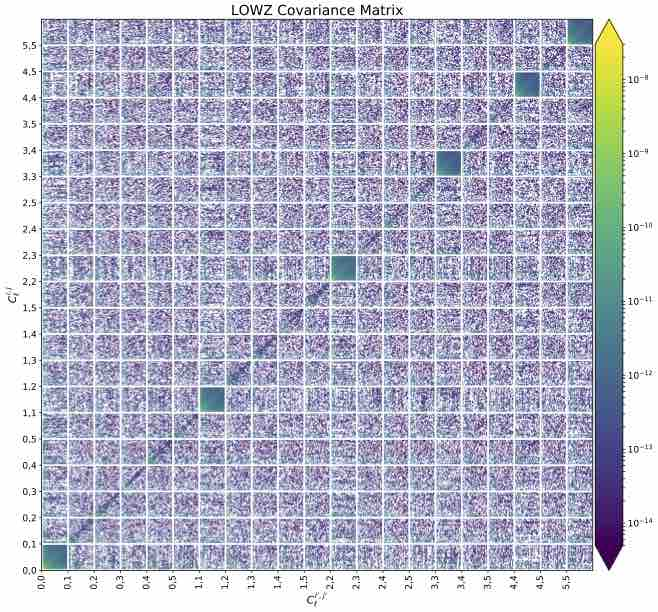
\includegraphics[width=1.\linewidth]{BOSS-FIGS/LOWZ_COV_Temp_TUAMAE.jpg}\label{fig:LOWZ_COV_Temp_TUAMAE.jpg}
% \end{subfigure}%
% \begin{subfigure}{.5\textwidth}
%   \centering
%   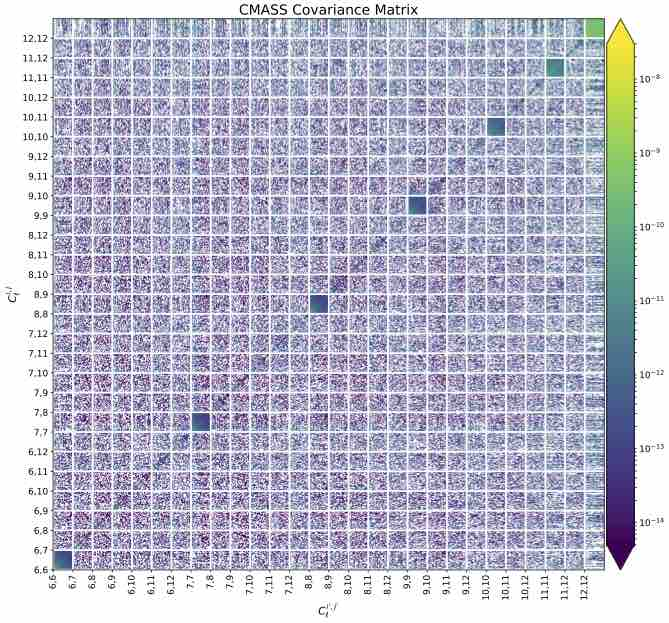
\includegraphics[width=1.0\linewidth]{BOSS-FIGS/CMASS_COV_Temp_TUAMAE.jpg}\label{fig:CMASS_COV_Temp_TUAMAE.jpg}
% \end{subfigure}
% \caption{Covariance matrices created with 6,000 \texttt{FLASK} log-normal simulations for \textit{(left)} LOWZ and  \textit{(right)} CMASS. The labels on the axis are the number (\textit{i,j}) of the redshift bins for covariance $\mathcal{C}(\hat{S}_{\Delta\ell}^{i,j},\hat{S}_{\Delta\ell'}^{i',j'})$.}
% \label{fig:CovMat}
% \end{figure}

\qquad To generate the mocks, I use \texttt{FLASK}\footnote{\url{http://www.astro.iag.usp.br/~flask/}} \citep{Flask2016}, a publicly available code that produces log-normal simulations of correlated fields in the sphere. Here, I use the data $\hat{S}_{\ell}$ measurements as inputs for the simulations (as measured in Section \ref{Sec:Measurements}). This technique allows me to reproduce any sort of systematic effects, RSD, non-linear power spectra, and other known and unknown effects that may be present in the data with no need to model them nor assume any fiducial cosmology. This is a main benefit of this approach to covariance estimation: any effects present in the measured angular power spectra will be reproduced in \texttt{FLASK}'s simulations via the $S_{\ell}$s measured from the data. 

\qquad For each of the samples, I produced 6,000 log-normal mocks to estimate the data covariance matrix. These mocks are also Poisson sampled to reproduce noise properties, radial and angular selection effects according to the data. 

\qquad The data covariance matrix was produced as follows:

\begin{enumerate}
\item[\textbf{1.}] Produce an spline, $\tilde{S}(\ell)$, using the $\hat{S}_{\Delta\ell}$ measurements (Figure \ref{fig:PCLs}) and a Gaussian filter to smooth the measurements.
\item[\textbf{2.}] Deconvolve the mixing matrix, $R_{\ell\ell'}$, from the splines to obtain
\begin{align}
\tilde{C}^{ij}(\ell) = \sum_{\ell'}R_{\ell\ell'}^{-1}\tilde{S}^{ij}(\ell)
%\label{Eq:Spline}
\end{align}
\item[\textbf{3.}] Monotonically extrapolate the splines to $\ell_{max} = 8192$ (necessary to allow \texttt{FLASK} to create high resolution \healpix maps).
\item[\textbf{4.}] For each tomographic redshift bin, produce \texttt{FLASK} partial sky galaxy number count mocks with $N_{side} = \ell_{max} = 2048$.\footnote{The signal realisation maps were sampled using a log-normal transformation. Due to the transformation's non-linearity, I had to generate mocks with a higher $N_{side} \quad \& \quad\ell_{max}$ than the data as the log-normal realisations introduce a damping after a certain $\ell$ (see figure 18 from \cite{Flask2016}). The simulated data maps also used a $N_{side}=2048$ version of the masks presented in \ref{Sec:Masks}.}
\item[\textbf{5.}] Degrade the mocks to $N_{side}=512$ to match the $N_{side}$ used when analysing the data.
\item[\textbf{6.}] Produce up-weighted overdensity maps (as described in section \ref{Sec:Maps}).
\item[\textbf{7.}]Run the partial sky PCL estimator; include here the pixel window function correction $w_{\ell}^2$ (as described in Equations \eqref{Eq:Sl_wl} and \eqref{Eq:S_delta_ell}) that arises from the degrading of the maps at step \textbf{5}.
\item[\textbf{8.}] Measure the covariance of the ensemble of angular power spectra obtained from the simulated data:
\begin{equation}
\mathcal{C}^{ij}_{\Delta\ell\Delta\ell'} \equiv \frac{1}{N_S-1}\sum^{N_S}_{s=1}\left(S_{\Delta\ell}^{ij,s} - \langle S_{\Delta\ell}^{ij} \rangle \right)\left(S_{\Delta\ell'}^{ij,s} - \langle S_{\Delta\ell'}^{ij} \rangle \right)^T.
\label{Eq:Covariance}
\end{equation}
\end{enumerate}
Here $N_S$ is the number of simulations.
To validate the estimated covariance matrix, I compared the diagonal of the covariance matrix in Equation \eqref{Eq:Covariance} with the expression for the theoretical variance for the measured angular power spectra in Equation \eqref{Eq:TheoVariance}; Figure \ref{fig:Mocks_Variance} shows a typical result.

\section{Systematic Null Tests}\label{Sec:Systm}
Large-scale survey observations, spread over thousands of observation hours, are taken under a variety of conditions. Turbulence in the atmosphere, sky background brightness and telescope inclination angle are amongst the factors that can influence image quality and object detection. Other than those atmospheric effects, galactic properties are also at play: extinction from dust within the Milky Way and variations of stellar density, as well as the presence of bright stars, are position-dependant and also have an impact on our ability to detect galaxies. Jointly, these observational factors have the potential to create small density fluctuations in the galaxy distribution which can imprint a statistical signal easily confused with the cosmological large-scale structure fluctuations that one is attempting to measure. This effect has been detected and corrected for in several previous analyses with a range of datasets \citep{Blake2007, 2011MNRAS.417.1350R, Thomas2011, Boris2013, Ho2012, Doux2017}.

\qquad In this section, I present the analysis performed on the data to ensure that the measured power spectra are not significantly dominated by any known observational systematic effects. I consider a systematic to have a significant effect on the observed power spectra if the cross-power spectra between them deviates from zero, with a deviation that is bigger than both the data variance and the cross-power spectra variance. I start by describing the systematic effects considered in this analysis, describing the methods for map creation and cross-spectrum measurement, and giving some representative results. Plots showing the complete analysis of systematics contamination for all 13 tomographic bins can be found in Appendix \ref{Apx:Systematics}.

%------------------------------------------------------------------------%
%                        	SYSTEMATICS MAPS
%------------------------------------------------------------------------%
\subsection{Systematic Maps}\label{Sec:SystMaps}

The Sloan Digital Sky Survey monitors and records observational conditions for every tile of the survey. This information is available as a combined set of two files, one that defines a pixelisation of the observed sky in \mangle format and another that records the observational information for each \mangle polygon.\footnote{The files, \texttt{window\textunderscore unified.fits} and \texttt{window\textunderscore flist.fits}, can be found in \url{http://www.sdss.org/dr12/algorithms/resolve/}, together with a detailed description of the construction of the survey geometry and of the \texttt{score} quantity described further in the text.} The first step is to reconstruct the \mangle maps for each observational systematic from these files. The \mangle python wrapper\footnote{\url{https://github.com/mollyswanson/manglepy}} was used to perform this transformation. Since there is potentially more than one observation in a given region of the sky, there can be multiple values for a given polygon. The SDSS files indicate which amongst multiple options is to be taken as the primary value for the field. The IDs were selected from those primary fields, matched to their observational properties in the fields list, and a new \mangle mask was created for each of those properties, which are recorded in the weight of the masks.

\qquad Next, \texttt{Mangle} masks were created for sky background flux, sky variance and average PSF FWHM in all five photometric bands. Mask of the \textit{score} of each field were also created -- defined by the SDSS collaboration to express ``observational quality" as an empirical combination of observational values with processing status flags. Additional observational properties can be found in the Field Table, available from the SDSS SkyServer Schema Browser.\footnote{\url{http://skyserver.sdss.org/dr12/en/help/browser/browser.aspx}} The choice of which systematics to take into account is somewhat arbitrary, as there are correlations between observational properties that make information redundant \citep{Boris2013}. Stellar density and galactic extinction were also added to the systematics listed above, as those have been shown to correlate with galaxy density in several previous analyses \citep[e.g.][]{Thomas2011, ElvinPoole2017}.The bright star catalogue was created from the SDSS object catalogue with the following cuts:
\begin{eqnarray}
18 < r_{psf} < 19.5,\\ \nonumber
\text{type} = 6,\\
r_{psf} - r_{\text{model}} < 0.25,\nonumber
\end{eqnarray}
where the extinction-corrected magnitude cut ensures robust star selection \citep{Padm2007}, the type selection is the standard SDSS star-galaxy classifier\footnote{\url{http://www.sdss.org/dr12/algorithms/classify/}} and the magnitude-difference cut is an additional point-source selection performed by the \texttt{GAMA} survey \citep[e.g.][]{Christodoulou2012}. For galactic extinction, a \healpix map was created directly. For simplicity, a python implementation of extinction $E(B-V)$ value retrieval and map creation\footnote{\url{https://github.com/kbarbary/sfdmap}} was used to create such map. Finally, the original SFD scaling map \citep{Schlegel1998} was also used.

\qquad The \mangle masks created from the SDSS FITS files are not appropriately snapped, pixelised and balkanised, which breaks the local character of the \mangle procedure \citep{2008Mangle}. As a consequence, further operations suffer from impractically large processing times. All the steps of the \mangle pixelisation scheme were ran anew, which corrects whatever imperfections remained in the first pass. From these masks, full-sky \healpix maps at resolution $N_{side}=16384$ were created, which defines an angular scale much smaller than the average resolution of the mask features. For each observational systematic, the sub-resolution \healpix pixels were populated with values from the associated \mangle mask. The resulting \healpix maps encapsulate all the information contained in the original footprint description.

\qquad Once the \healpix systematics maps are created, the next step is to transform them into overdensity maps using the same procedure outlined in Section \ref{Sec:Maps} for the data \citep{Boris2013}. The idea is to treat the systematic maps in the same way as the data in order to apply the statistical estimators consistently. Therefore, I degrade the high-resolution maps to the data resolution ($N_{side} = 512$) and up-weight the maps according to the pixel completeness mask that takes the holes in the footprint into account (see Section \ref{Sec:Masks}); I then perform a cut in pixel completeness $C_{pix} = 0.8$ in the maps. From these post-processed maps, I create the systematics overdensity maps as: 
\begin{equation}
\delta_{i}^{Sys} = 
\begin{cases}
\left(\frac{1}{C_{pix,i}}\frac{n^{Sys}_{i}}{\bar{n}^{Sys}}\right) - 1 & \text{, if } C_{pix,i} \geq 0.8 \\
0 & \text{, otherwise}
\end{cases}
\label{Eq:OverDMapsSyst}
\end{equation}
where $n^{Sys}_{i}$ is the pixel value for a given systematic and $\bar{n}^{Sys}$ is the mean value of the map in the observed fraction of the sky. The systematics overdensity maps were created using both the CMASS and LOWZ masks presented in Section \ref{Sec:Masks}. The resulting systematics overdensity maps are shown in figure \ref{fig:SYS_Appendix1Map} and in figure \ref{fig:ExtincSys} for extinction using the CMASS mask as an example.

\begin{figure}
\begin{center}
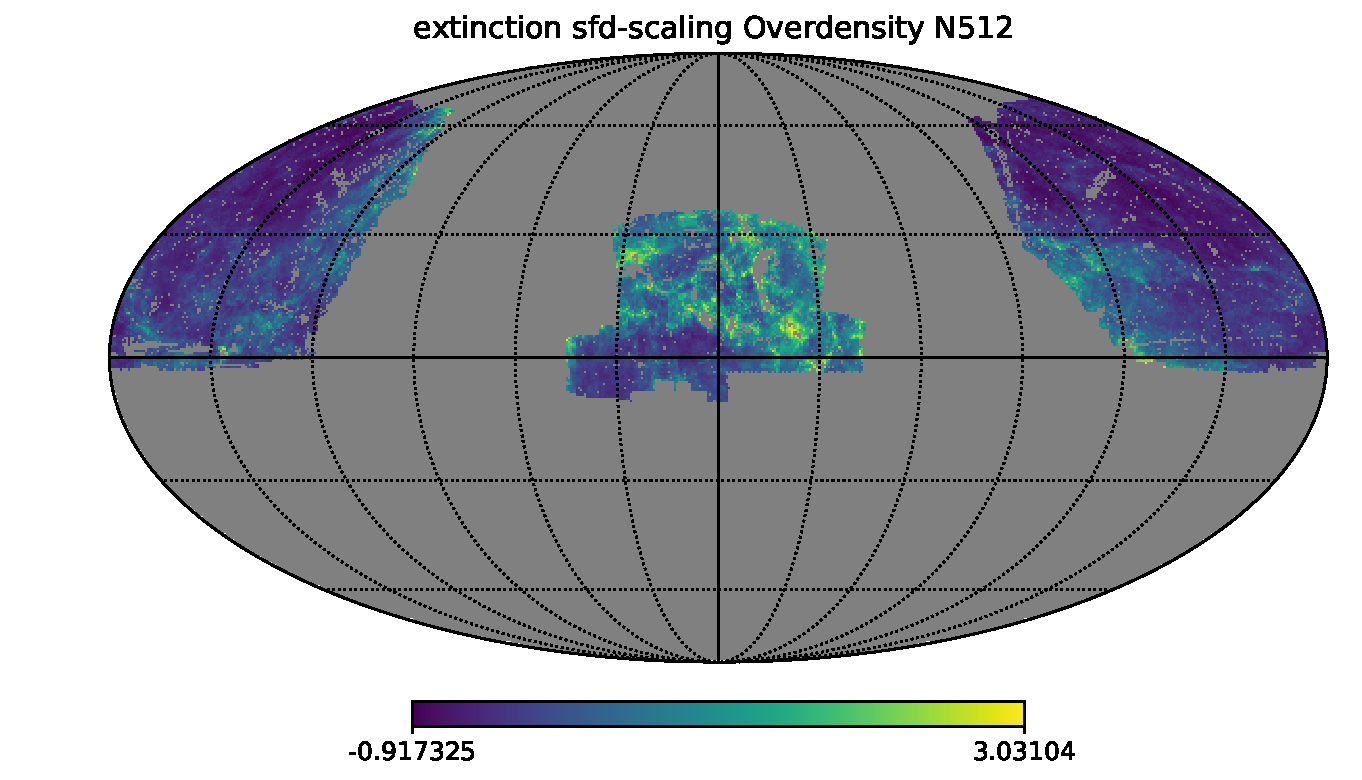
\includegraphics[width=\textwidth]{BOSS-FIGS/map_extinction_sfd-scaling_Overdensity_N512_cmassAll.pdf}
\caption[Extinction SDF scaling overdensity systematic map.]{An example of systematics overdensity maps from Section \ref{Sec:SystMaps}: the extinction sfd scaling map \citep{Schlegel1998} using the CMASS mask from Section\ref{fig:Masks}. }
\label{fig:ExtincSys}
\end{center}
\end{figure}

%------------------------------------------------------------------------%
%                        	SYSTEMATICS CROSS-CLS
%------------------------------------------------------------------------%
\subsection{Cross-power spectra between data and systematic maps:}\label{Sec:SystCls}
\begin{figure*}
\begin{center}
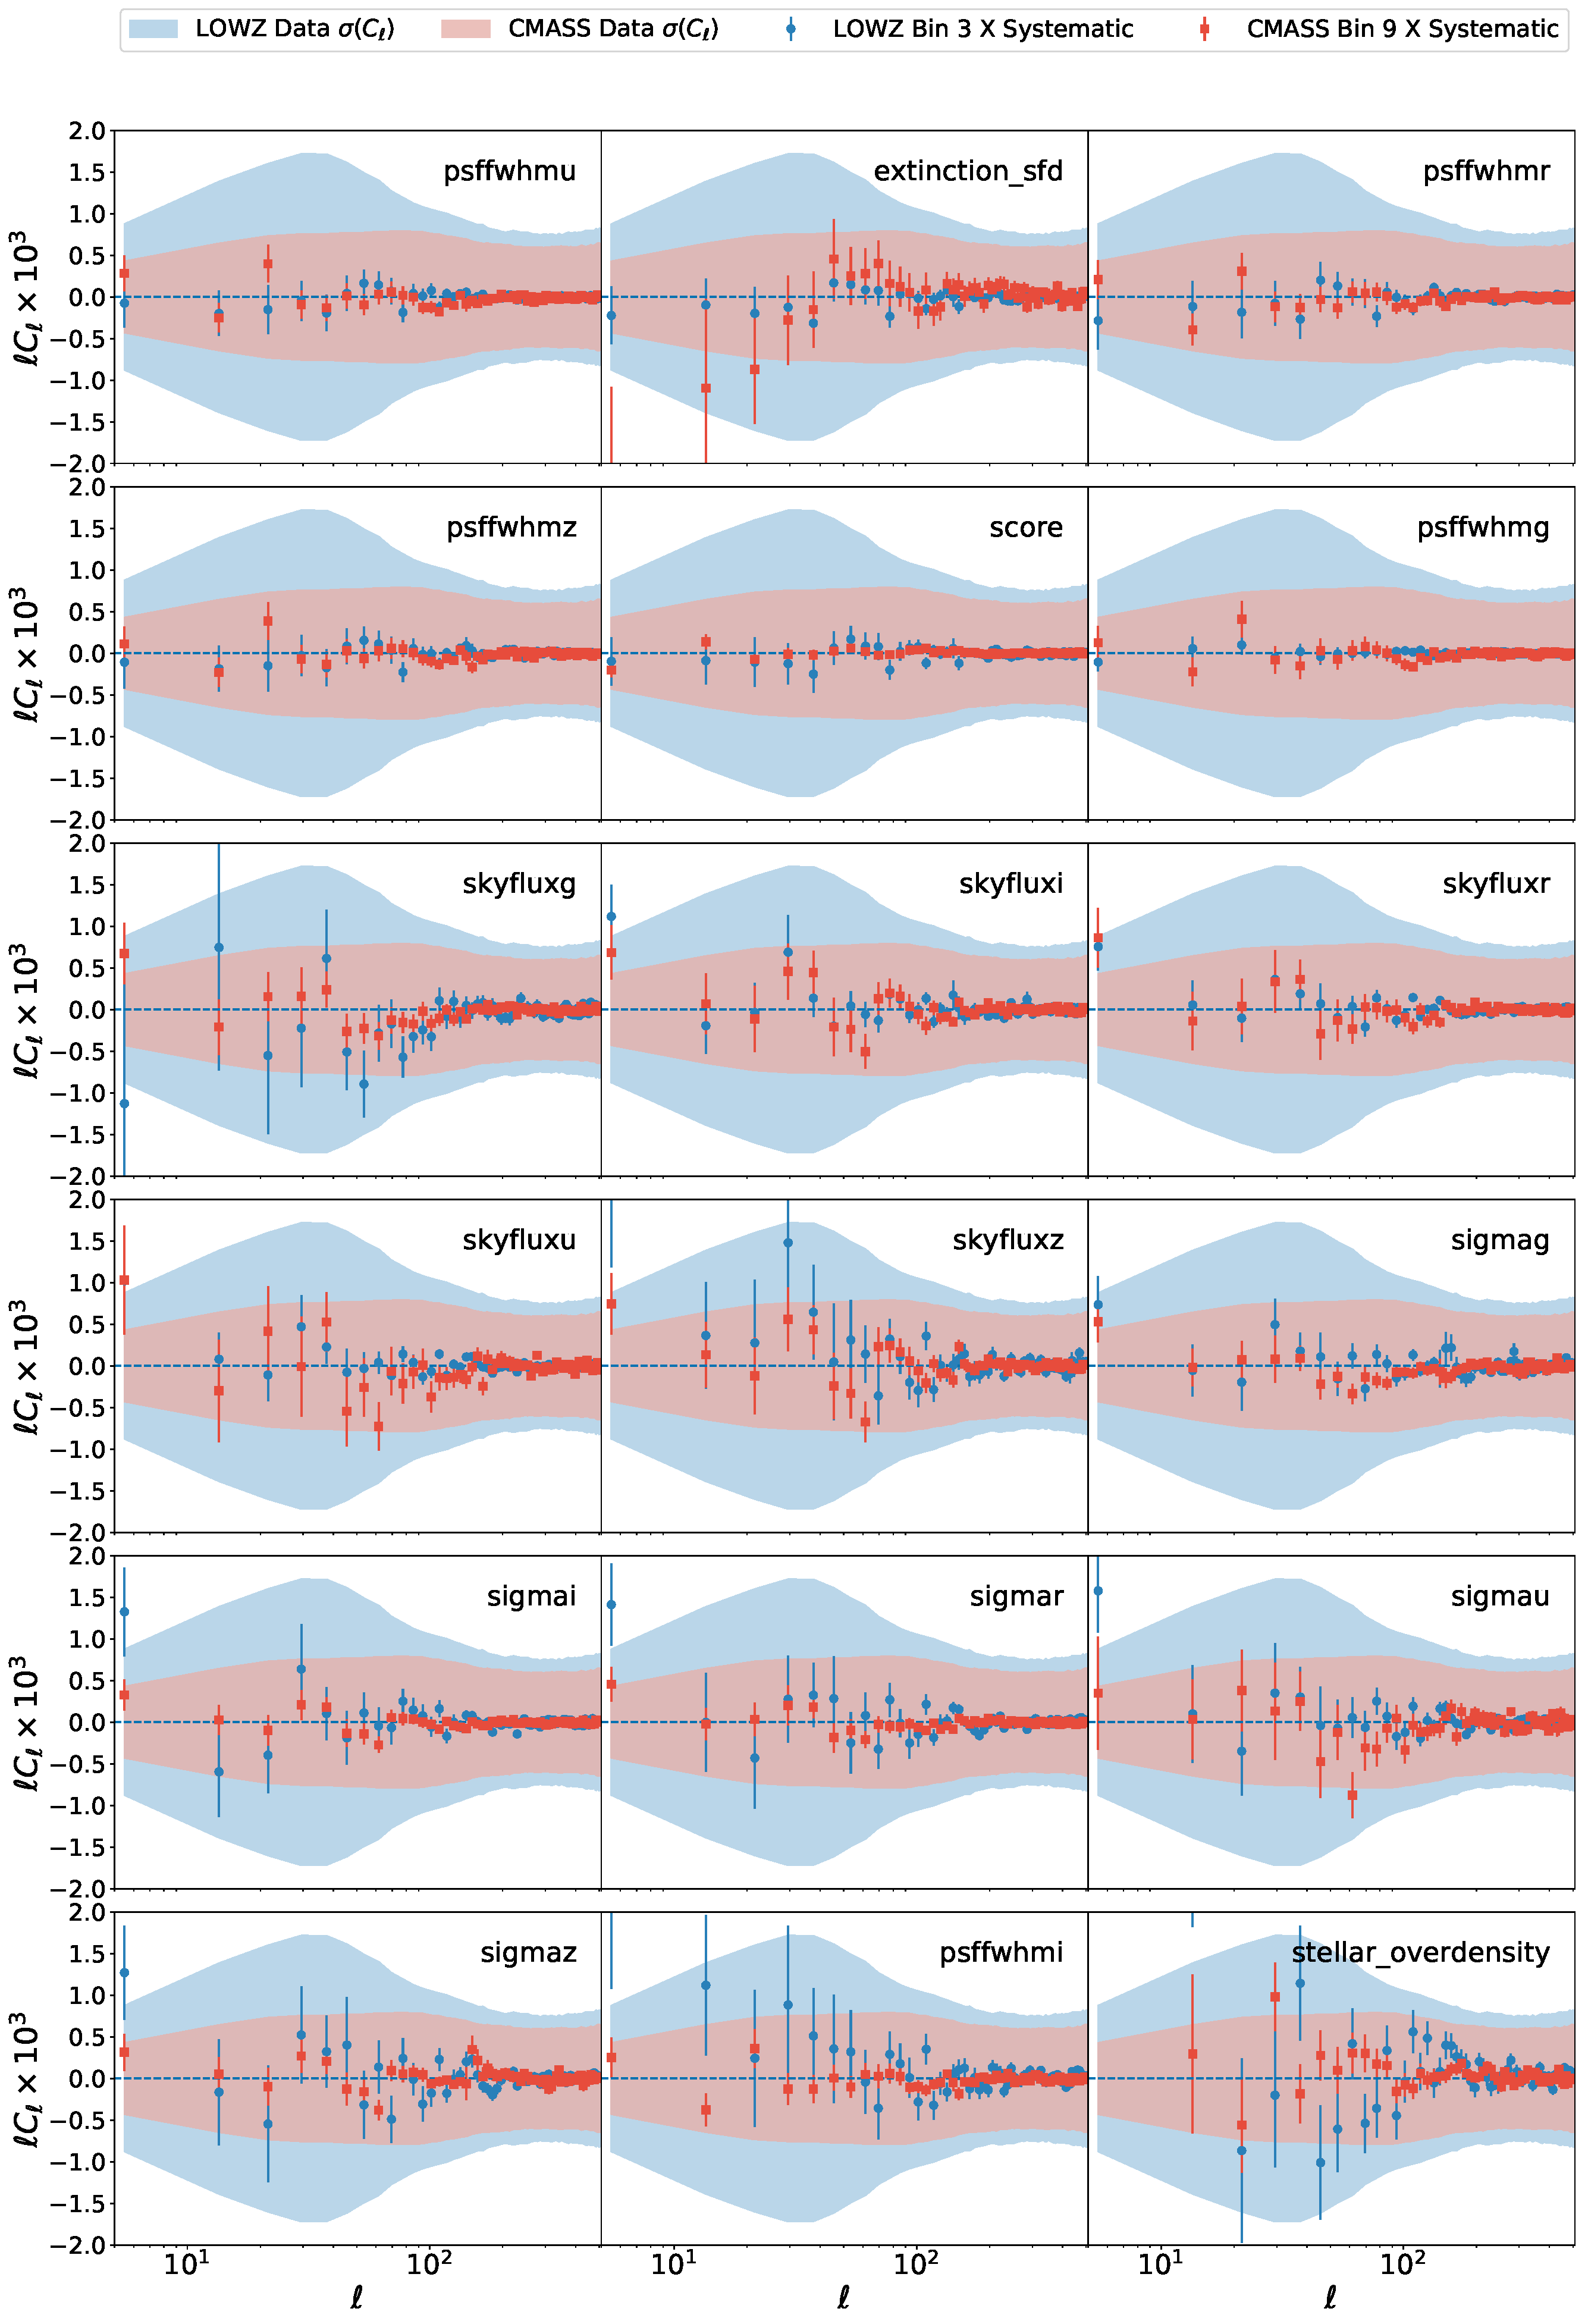
\includegraphics[scale=0.30]{BOSS-FIGS/systematics_CMASS_Bin3_LOWZ_Bin3.pdf}
\caption[An example of the systematics analysis for the BOSS samples.]{An example of the systematics analysis described in Section \ref{Sec:SystCls}. Here, I show the cross-power spectra between the 18 systematics overdensity maps produced in \ref{Sec:SystMaps}, and LOWZ--3 (CMASS--9) tomographic bins in blue dots (red squares). The error-bars were obtained by cross-correlating the $\delta^{Sys}$ maps with the \texttt{FLASK} mocks produced in Section \ref{Sec:Cov}; the shaded region shows the variance of the data, which was also obtained from the same mocks. This figure indicates that the shape of the measured power spectra in Figure \ref{fig:PCLs} is not dominated by any of the systematics considered, as the variance of the cross-power spectra between data and systematics is consistent with the variance of the data's auto-power spectra. The results for the other bins similar to the results shown in this figure and can be found in Appendix \ref{Apx:Systematics}. Note also that the first $\ell-$band in the stellar overdensity cross-$C_{\ell}$ is completely out of the acceptable range, which lead me to exclude this data point on all bins for both samples.}
\label{fig:SystBin3}
\end{center}
\end{figure*}
For the systematics analysis using cross-power spectra, I follow a data analysis in a similar fashion as the one performed for the galaxy overdensity maps in Section \ref{Sec:Measurements}.  Using Equation \eqref{Eq:AlmPix} I decompose the systematics overdensity maps, $\delta^{Sys}$, into spherical harmonics. 

The estimator for the cross-power spectra between the data overdensity maps, $\delta^{g}$, and the systematics can be written as a modified version of Equation \eqref{Eq:Sl_wl}:

\begin{equation}
\hat{S}^{gs}_{\ell} = \frac{1}{(2\ell+1)w_{\ell}^2}\sum_{m=-l}^l  \frac{\frac{1}{2}\left|d_{}^{g}  d_{\ell m}^{s*} + d_{\ell m}^{g*}  d_{\ell m}^{s}\right|}{J_{\ell m}}
\label{Eq:Sl_wlSyst}
\end{equation}
where the index \textit{g} stands for a data map, and \textit{s} for a systematics map. I then obtain the estimates for the variance of the systematics cross-power spectra by measuring the $\hat{S}^{gs}_{\ell}$ (Equation \eqref{Eq:Sl_wlSyst}) between the Systematics maps and the data mocks described in Section \ref{Sec:Cov}.

\qquad I cross-correlated all 13 tomographic redshift bins with all 18 systematic maps, resulting in a total of 234 cross-power spectra. Figure \ref{fig:SystBin3} shows an example for LOWZ--3 and CMASS--9 bins and cross-power spectra for all systematics. The full results are shown in Appendix \ref{Apx:Systematics}. From all of these, the majority of measurements are consistent with the variance of the data measured from the log-normal simulation (Section \ref{Sec:Cov}), which lead me to be confident in using the full shape of the measured $C_{\ell}$s. Note, however, that a few of the large scale measurements (low-$\ell$) in CMASS sample have a small excess in cross-power spectra with stellar overdensity. The first point on the cross-power spectra between some of the systematic maps and most BOSS bins is clearly more than one sigma away from the data's variance. Due to this excess in correlation with stellar overdensity and the level of cosmic variance on the first $\ell$-band, I decided to exclude this first point from the cosmological analysis (see Chapter \ref{Chap:BOSS-Cosmo} for details on the $\ell$ range used). As for the second $\ell$-band ($\ell = 13.5$) presenting an excess of correlation between a few bins and stellar overdensity: I found it to be sub-dominant, with no significant impact from this measurement in our cosmological analysis; therefore, I decided to keep it.

\section{Conclusions}\label{Sec:Concl1}
%In this chapter, I presented the process towards building a full data-vector for the BOSS DR12 large scale structure sample using a harmonic space approach. Given the spectroscopic nature of the data-set, I was able to divide it into 13 redshift tomographic bins with an equal size ($\Delta z = 0.05$). This
In this work, I have taken a different approach\footnote{Compared to the approaches from the official BOSS Collaboration papers: \cite{2017RossBOSS,2017BeutlerBOSS,2017Beutler2BOSS,2017SatpathyBOSS,2017SanchezBOSS,2017GriebBOSS,2017SalazarBOSSwTheta,2017WangBOSS,2017ZhaoBOSS}.} to obtain galaxy clustering information from the BOSS DR12 large scale structure catalogue \citep{BOSSCatalogue2016}. This approach consisted in using a pseudo angular power spectra estimator (PCL) applied to 13 tomographic redshift bins ranging from $0.15 \leq z < 0.8$ with a redshift dependent bias, a redshift dispersion, and extra shot-noise as nuisance parameters to be sampled with the cosmological parameters using \uclcl (Cuceu et al., \textit{in prep}). In this approach, I have used splines of the data as input for the simulation used for covariance matrix estimation.

\qquad The tomographic analysis in redshift space and the covariance matrix estimation method used in this work allow for cosmology-free inference to be performed from the data. In other words, in no moment in this analysis a fiducial cosmology was assumed. This is, by itself, a great advantage over methods that use $P(k)$ or $\xi(r)$ as these need to assume a fiducial cosmology in order to transform from redshift space to radial distances. The impact of such strong assumption in the cosmological inference is still unknown.

\qquad I performed systematic contamination checks with the data with satisfactory results. From the 18 different sources of systematic considered in Section \ref{Sec:Systm}, none demonstrated worrying excess of power in the scales considered (with the exception of the first bandwidth, $\Delta \ell = [2,10]$). Although some other $\ell$-modes do present a small excess of clustering with, for example, stellar overdensity, these were not found to have a significant impact on the overall clustering of galaxies when compared to the intrinsic variance of the data -- estimated from the log-normal simulations.

\qquad Finally, I have constructed a data-vector and covariance matrices from a spherical harmonic analysis of BOSS DR12 galaxies which are cosmology-free, i.e. no fiducial model was assumed at any moment in this analysis. With the theoretical framework detailed in Section \ref{Sec:Theory}, these measurements are now ready to be used in a cosmological posterior analysis to infer cosmological parameters. The next Chapter performs some additional checks in the methodology and data-vector outlined here; subsequently probing the main cosmological models and demonstrating the full constraining power of the data-vector produced in this Chapter.